\documentclass[a4paper,12pt]{article}
\usepackage{../styledoc19}


\begin{document} % конец преамбулы, начало документа
	
	\itsHSE
	\academicTeacher{Преподаватель департамента \vfill программной инженерии  факультета компьютерных наук}
	{М. К. Горденко}
	
	\projectName{IOS-ПРИЛОЖЕНИЕ <<СОЦИАЛЬНАЯ СЕТЬ ДЛЯ СОТРУДНИКОВ НИУ ВШЭ>>}
	
	\titleList{Руководство оператора}{RU.17701729.04.03-01 34 01-1}
	\par\vspace{60mm}
	\nameOfAuthor{БПИ174}{Д. Ю. Редникина}
	\tabForFirstPage
	
						\newpage
	
	\pagestyle{fancy}
	\lhead{УТВЕРЖДЕН \newline
	 	RU.17701729.04.03-01 34 01-1}
	\vspace*{\fill}
	\begingroup
	\centering
	\tabForFirstPage
	\projectName{IOS-ПРИЛОЖЕНИЕ <<СОЦИАЛЬНАЯ СЕТЬ ДЛЯ СОТРУДНИКОВ НИУ ВШЭ>>}
	\titleList{Руководство оператора}{RU.17701729.04.03-01 34 01-1}
	\listNumber{22}
	
	\endgroup
	\vspace*{\fill}
	
	
						\newpage
	\lhead{ }
	\chead{\vfill \thepage \vfill  RU.17701729.04.03-01 34 01-1}
	\rhead{ }
	\cfoot{ }
	%delete this if you are not writing a TZ
	\cfoot{\tabForTZ}
	\tableofcontents
	\newpage
	\section{Назначение программы}
	\subsection{Функциональное назначение }
	Программа применяется как средство коммуникации между сотрудниками НИУ ВШЭ. Сервис также позволяет сотрудникам НИУ ВШЭ координировать совместные исследования и проекты научного характера. Приложение предоставляет доступ к общению посредством сообщений, дает возможность делиться новостями с помощью публикации постов. Также приложение дает возможность фильтровать новости по интересущим темам. 

	\subsection{Эксплуатационное назначение}
	% ЭКСПЛУАТАЦИОННОЕ НАЗНАЧЕНИЕ

Программа будет использоваться как средство общения и огранизации работы над совместными научными проектами между сотрудниками с одного или разных направлений/ факультетов/ кампусов. 


Таким образом, программный продукт позволит решить проблему коммуникации между факультетами, кампусами НИУ ВШЭ и даст возможность наладить взаимодействие между преподавателями университета, будет способствовать развитию научной деятельности между разными факультетами и кампусами.
	\subsection{Состав выполняемых функций}
	% требования
% dyurednikina
% version 1.2
% last modified 7.05.2019


Программа выполняется в рамках темы курсовой работы в соответствии с учебным планом подготовки бакалавров по направлению 09.03.04 «Программная инженерия» Национального исследовательского университета «Высшая школа экономики», факультет компьютерных наук.

Разработка требований велась совместно с командой и заказчиком в рамках предмета <<Групповая динамика и коммуникации в программной инженерии>>



\textit{Состав команды}:
\begin{itemize}
	\item Анна Михалева - android-developer;
	\item Константин Манежин - web-developer;
	\item Илья Костюченко - backend-developer;
	\item Дарья Редникина - iOS-developer;
\end{itemize}


\textit{Заказчик}:
\begin{itemize}
	\item Девятьярова Анна Дмитриевна, Факультет бизнеса и менеджмента/ 
	Кафедра управления человеческими ресурсами.
\end{itemize}
% \subsection{Клиентские приложения}
%\renewcommand{\labelenumi}{FR-\arabic{enumi})}
\renewcommand{\labelenumi}{\textbf{FR-\arabic{enumi}}.}

\renewcommand{\labelenumii}{\textbf{FR-\arabic{enumi}.\arabic{enumii}}.}

\renewcommand{\labelenumiii}{\arabic{enumiii}.}

\begin{enumerate}
	\item \textbf{Авторизация клиента\\}
	Чтобы использовать программу, клиент должен иметь возможность авторизоваться в системе.
	\begin{enumerate} \label{req: auth}
		\item При регистрации в социальной сети клиенту необходимо заполнить обязательные поля регистрации: \label{FR-1.2}
		\begin{enumerate}
			\item (\textit{Verified, автор: заказчик}) \\ФИО;
			\item (\textit{Verified, автор: заказчик}) \\Факультет;
			\item (\textit{Verified, автор: заказчик})\\Почта;
			\item (\textit{Verified, автор: заказчик})\\Должность; 
			\item (\textit{Verified, автор: заказчик})\\Город; 
		\end{enumerate}
		\item (\textit{Verified, автор: Илья})\\Уже зарегистрированный клиент для входа в социальную сеть должен ввести свою почту с доменом \verb+@hse.ru+.
		\item (\textit{Verified, автор: Анна})\\
		После успешной авторизациии/регистрации пользователю будет выслан код на введенную им почту, который нужно ввести в специальное поле в приложении, только после правильного ввода кода клиент сможет войти в социальную сеть.
	\end{enumerate}
	\item \textbf{Просмотр профиля пользователя}
	\begin{enumerate}
		\item (\textit{Verified, автор: Дарья})\\Должна быть возможность редактирования у пользователей выше перечисленных полей (см. требование \nameref{FR-1.2}), заполненых при регистрации, в настройках профиля. 
		\item (\textit{Verified, автор: команда, Анна})\\
		На странице профиля должна быть возможность просмотра раннее опубликованных постов человека. 
		\item (\textit{Verified, автор: Константин, заказчик})\\ 
		Также на странице должна быть возможность просмотра личных данных пользователя, то есть информации из требования \nameref{FR-1.2}
		\item (\textit{Verified, автор: Анна})\\
		На странице пользователя должна быть возможность написать сообщение пользователю в диалог.
		\item (\textit{Verified, автор: Анна})\\
		На странице пользователя должна быть возможность добавить пользователя в существующий канал.
	\end{enumerate}
	\item \textbf{Публикация постов\\} 
	Клиент имеет возможность опубликовать текстовую информацию от своего имени, чтобы она отображалась в ленте у других пользователей приложения и у него в профиле.
	\begin{enumerate}
		\item (\textit{Verified, автор: Илья})\\
		При написании поста у пользователя есть возможность добавить хэштеги к текстовой информации.
		\begin{enumerate}
			\item Хэштеги должны состоять из одного слова
			\item Хэштеги должны состоять из латинских и русских букв, допустимые символы при написании хэштега: нижнее подчеркивание, цифры.
			\item При неверном формате введенного хэштега он не будет опубликован вместе с написанным постом.
		\end{enumerate}
		\item (\textit{Verified, автор: Константин})\\
		При выборе хэштегов пользователю должны предлагаться autosuggested hashtags, раннее использованные в приложении другими пользователями при публикации постов.
		\item (\textit{Verified, автор: Анна})\\
		Должна быть поддержка разметки markdown, syntax highlighting при написании поста. 
		\item (\textit{Verified, автор: Дарья})\\
		При выходе из раздела создания поста, должна быть возможность сохранить черновик с текущем текстом и набором хэштегов. 
	\end{enumerate}
	\item \textbf{Лента\\}
	Пользователь должен имеет возможность, находясь в ленте, совершать поиск по интересущим его хэштегам, смотреть новости.
	\begin{enumerate}
		\item (\textit{Verified, автор: Дарья})\\
		При входе в основную ленту должна быть возможность отображения всех существующих постов только в хронологическом порядке.
		\item (\textit{Verified, автор: Константин}) \\ 
		Должна быть возможность осуществления перехода при нажатии на какой-либо хэштег в ленту всех постов с выбранным хэштегом. 
		\item (\textit{Verified, автор: Илья})\\
		Должна быть возможность подсказки autosuggested hashtags при поиске нужной информации в поисковой строке в ленте. 
		\item (\textit{Verified, автор: Илья})\\
		Должна быть возможность отображения как preview поста в ленте, так и его полного содержания в отдельном окне при нажатии. 
		\item (\textit{Verified, автор: Анна})\\
		Должна быть возможность перехода на страницы авторов постов, отображенных в ленте. 
		
	\end{enumerate}
	\item \textbf{Каналы [\ref{term: channel}] \\}
	У клиента приложения должна быть возможность сохранять поисковые фильтры для быстрого доступа к просмотру ленты по нужному множеству хэштегов и людей.
	\begin{enumerate}
		\item (\textit{Verified, автор: Константин}) \\
		Должна быть возможноть создания канала, который должен иметь:
		\begin{enumerate}
			\item Название;
			\item Еединое множество людей и хэштегов; 
			\item Функцию <<предпросмотр канала>>;
		\end{enumerate}
		\item (\textit{Verified, автор: Дарья}) \\
		Должна быть возможноть редактирования каналов, где можно:
		\begin{enumerate}
			\item Изменить название канала;
			\item Изменить множество выбранных хэштегов и людей;  
			\item Перейти к предпросмотру канала;
		\end{enumerate}
		\item (\textit{Verified, автор: Константин}) \\
		Должна быть возможность автоподсказки по хэштегам при редактировании канала; 
		\item (\textit{Verified, автор: заказчик, Анна}) \\
		Просмотр содержимого канала;
		\item (\textit{Verified, автор: Константин}) \\
		Удаление каналов;
		\item (\textit{Verified, автор: Анна})\\ 
		Должна быть возможность поиска по названию созданных каналов;
	\end{enumerate}
	\item \textbf{Создание чатов для пользователей\\}
	Клиент должен иметь возможность общаться с другими пользователями социальной сети: обмениваться сообщениями в диалогах и групповых беседах.
	\begin{enumerate}
		\item (\textit{Verified, автор: Анна, заказчик})\\
		Должна быть возможность создать групповую беседы (добавление участников, названия чата) размером от 2 до 50 пользователей
		\item (\textit{Verified, автор: Илья})\\
		При правах администратора беседы клиент должен иметь возможность:
		\begin{enumerate}
			\item Менять состав участников: добавлять или удалять;
			\item Менять название;
			\item Делать администраторами других людей из беседы;
			\item Лишать их возможности быть администратором; 
		\end{enumerate}
		\item (\textit{Verified, автор: Дарья})\\
		Создатель беседы автоматически должен являться администратором.
		\item (\textit{Verified, автор: Константин})\\
		Должна быть возможность просматривать информацию о беседе (состав участников, название беседы, список администраторов).
		\item (\textit{Verified, автор: Илья})\\
		Должна быть возможность выйти из беседы. 
		\item (\textit{Verified, автор: Дарья})\\
		Должна быть возможность написать сообщение другому пользователю. 
	\end{enumerate}
	\end{enumerate}

\renewcommand{\labelenumi}{\arabic{enumi}.}

\renewcommand{\labelenumii}{\arabic{enumii}.}

\renewcommand{\labelenumiii}{\arabic{enumiii}.}

	
	\newpage
	\section{Условия выполнения программы}
	\subsection{Минимальный состав аппаратурных средств}
	Для надежной и бесперебойной работы программы требуется следующий состав аппаратурных средств:
	
	\begin{enumerate}
		\item Персональный компьютер фирмы \textit{Apple} ;
		\item Мобильное устройство iPhone;
		\item 150 МБ оперативной памяти или больше;
		\item Не менее 1ГБ свободного места на жестком диске;
		\item Трекпад или мышь;
	\end{enumerate}

	\subsection{Минимальный состав программных средств}
	Для надежной и бесперебойной работы программы требуется следующий состав программных средств:
	\begin{enumerate}
		\item Должна быть установлена операционная система iOS 12.2 или новее. \item На компьютере пользователя должен быть установлен \textit{Xcode} 10.2.
	\end{enumerate}
	\subsection{Требования к персоналу}
	Для работы с данным приложением пользователь должен обладать базовыми знаниями работы социальных сетей и работы операционной системы iOS.
	
	\newpage 
	\section{Выполнение программы}
	\subsection{Загрузка и запуск программы}
	После распаковки архива \textit{dyurednikina.zip} содержимое папки \textit{GDproject} будет выглядеть следущим образом (см. рис \ref{pic: Folder}):
		\begin{figure}[h]
		\centering
		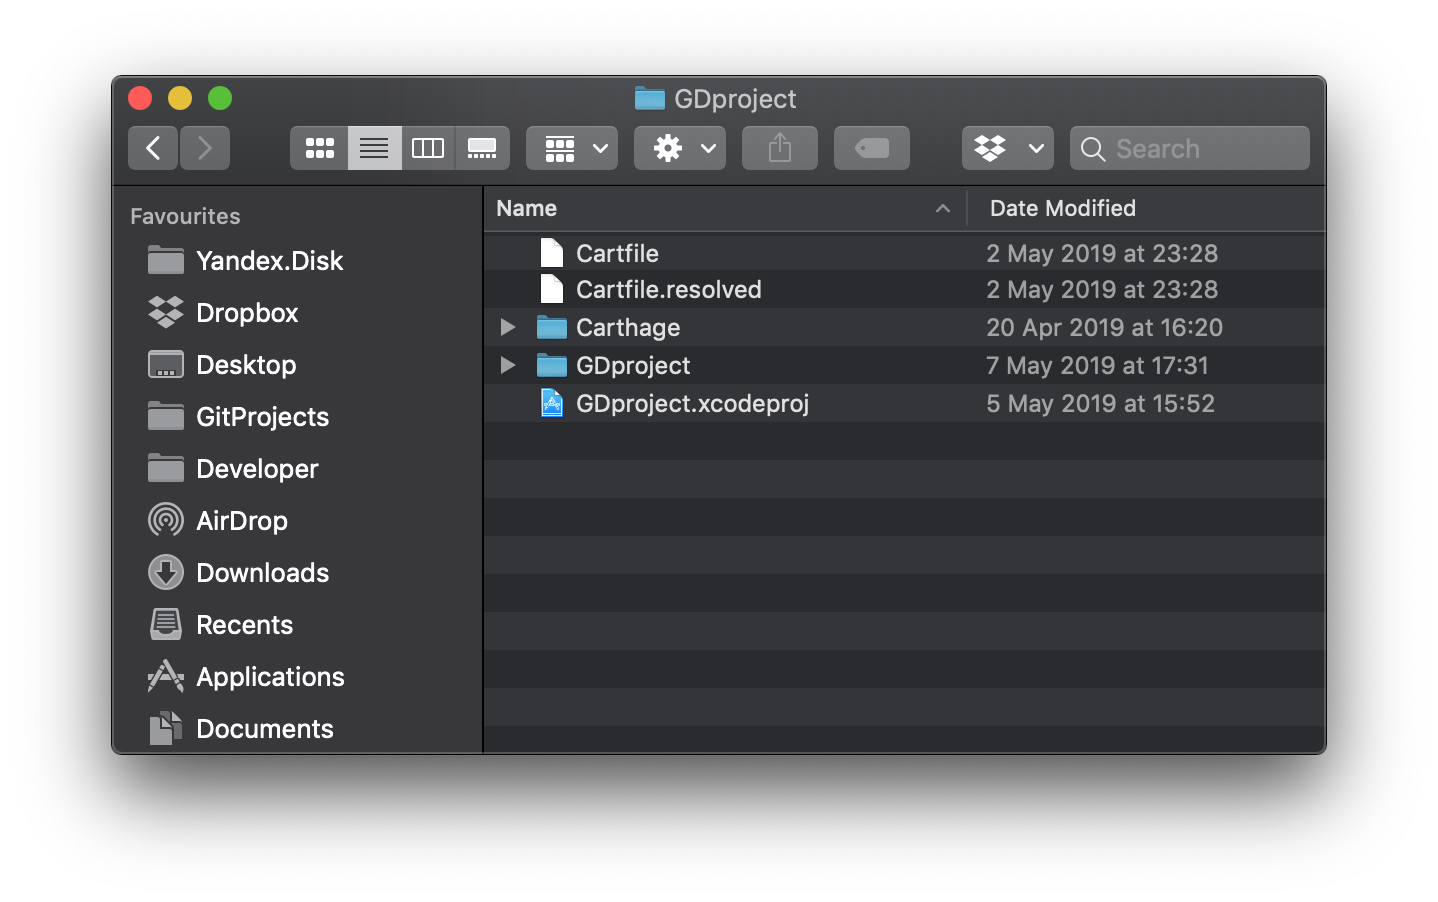
\includegraphics[width = \linewidth]{../includes/ro/folder.png}
		\caption{Папка, содержащая проект}
		\label{pic: Folder}
	\end{figure}


	Для запуска программы через симулятор или мобильный телефон требуется открыть файл \textit{GDproject.xcodeproj}, заранее установив программу \textit{Xcode} через магазин \textit{App store}. 
	
	Для запуска проекта требуется выбрать модель симулятора или подключенное к ноутбуку устройство и нажать \textit{Play} (см. рис \ref{pic: Play}).
	
	\begin{figure}[h]
		\centering
		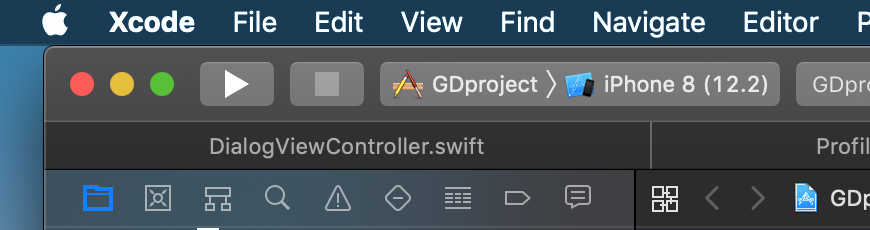
\includegraphics[width = 0.6\linewidth]{../includes/ro/play.png}
		\caption{Запуск проекта}
		\label{pic: Play}
	\end{figure}
	
	\subsection{Выполнение программы}
	\subsubsection{Регистрация}
	При входе в аккаунт пользователю предлагается ввести свою почту (см. рис \ref{pic: register}):
	Процесс регистрации:
		\begin{enumerate}
			\item Ввод email -- происходит отправка запрос на сервер для валидации данных
			\item При успешной валидации почты на сервере, происходит получение письма на введенную почту с кодом подтверждения 
			\item Клиент вводит полученный код в специальное поле 
			\item Открывается окно с регистрацией: пользователю необходимо заполнить обязательные поля (см. раздел требований \ref{req: auth})
			\item После заполнения пользователь подтверждает создание учетной записи и клиент успешно входит в приложение
		\end{enumerate}
	\begin{figure}[h!]
		\centering
		\begin{subfigure}[b]{0.3\linewidth}
			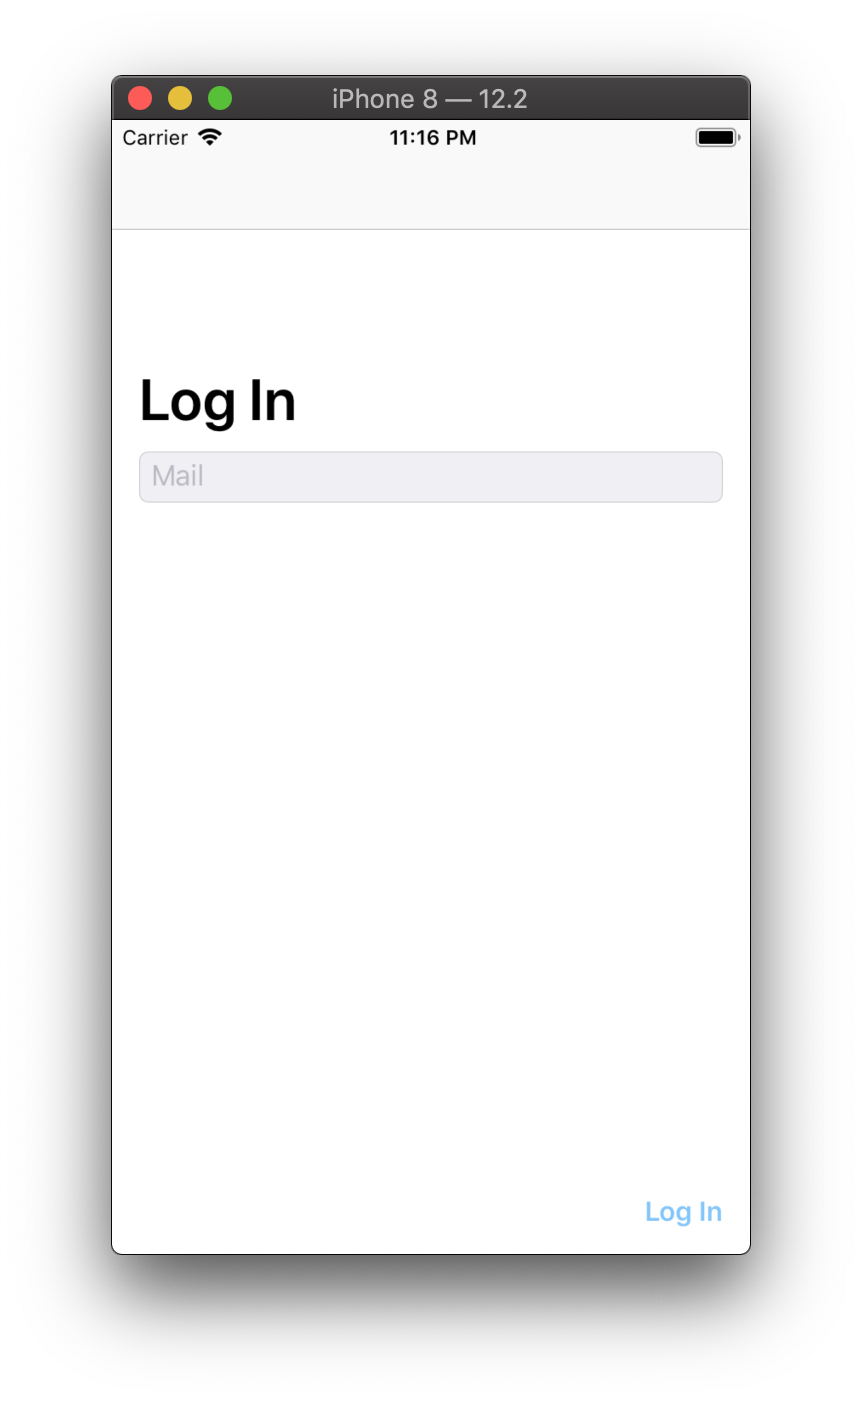
\includegraphics[width=\linewidth]{../includes/pmi/login.png}
		\end{subfigure}
		\begin{subfigure}[b]{0.3\linewidth}
			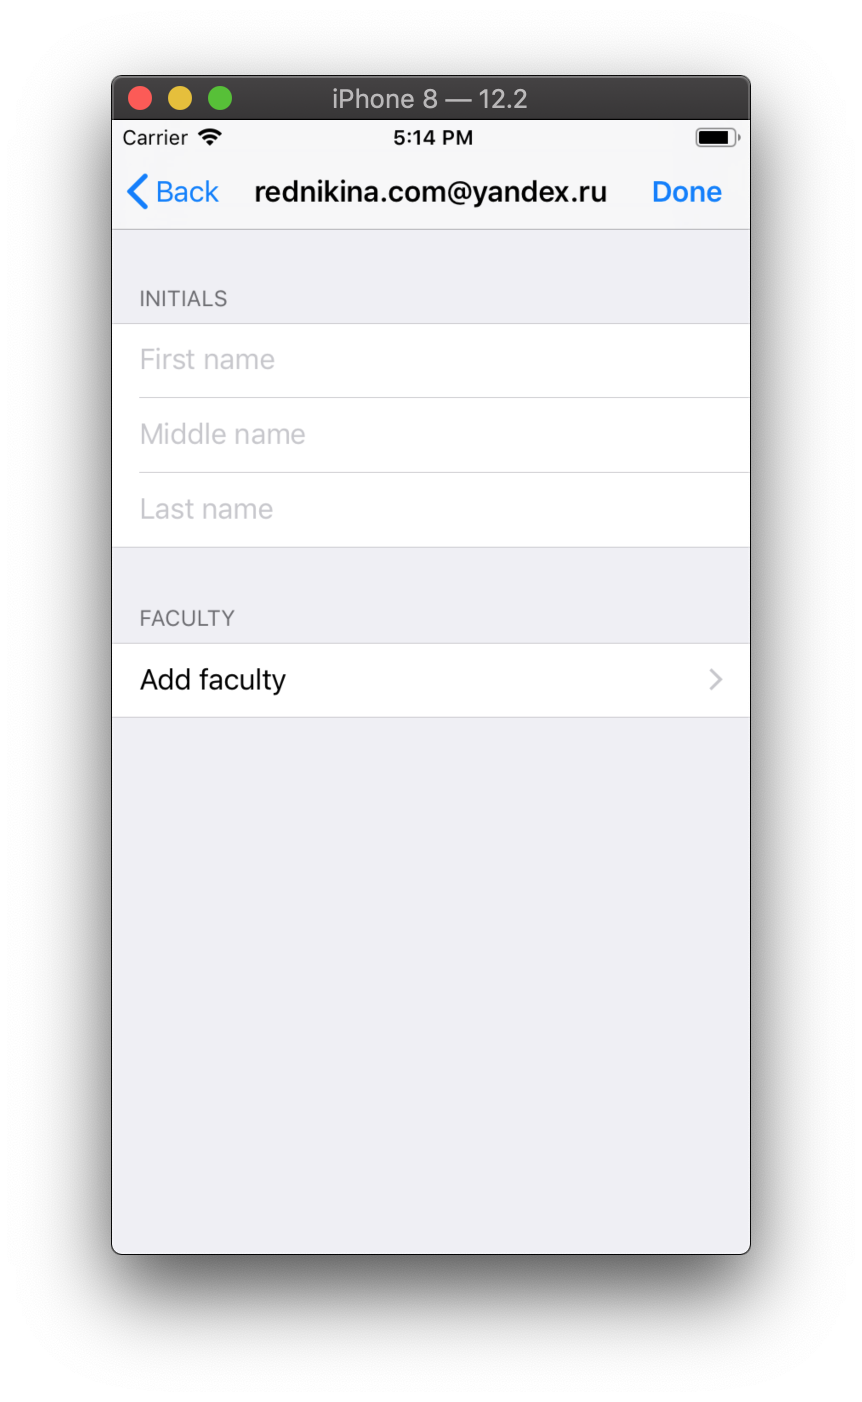
\includegraphics[width=\linewidth]{../includes/pmi/r1.png}
		\end{subfigure}
		\begin{subfigure}[b]{0.3\linewidth}
			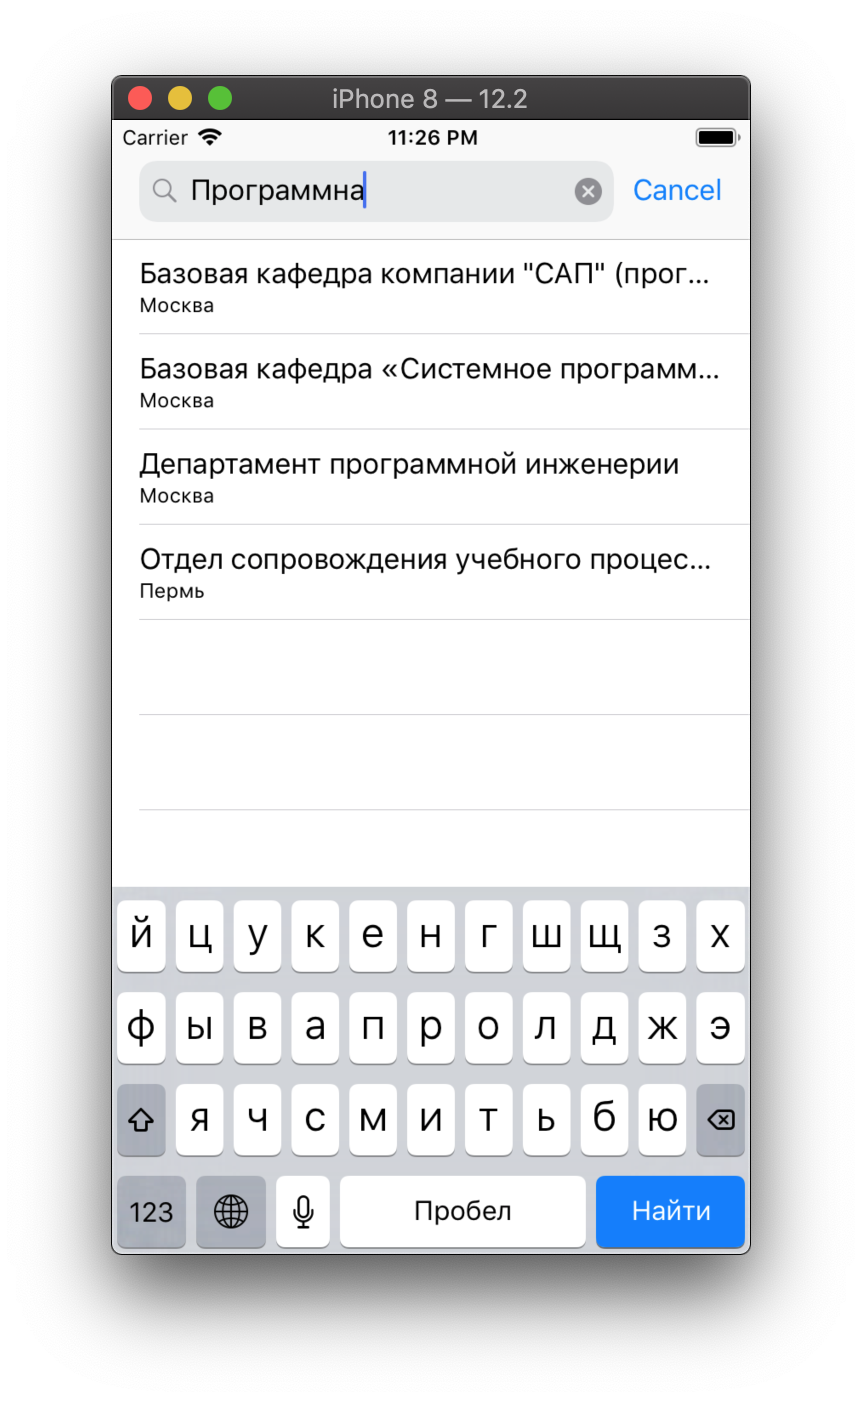
\includegraphics[width=\linewidth]{../includes/pmi/r3.png}
		\end{subfigure}
		\begin{subfigure}[b]{0.3\linewidth}
			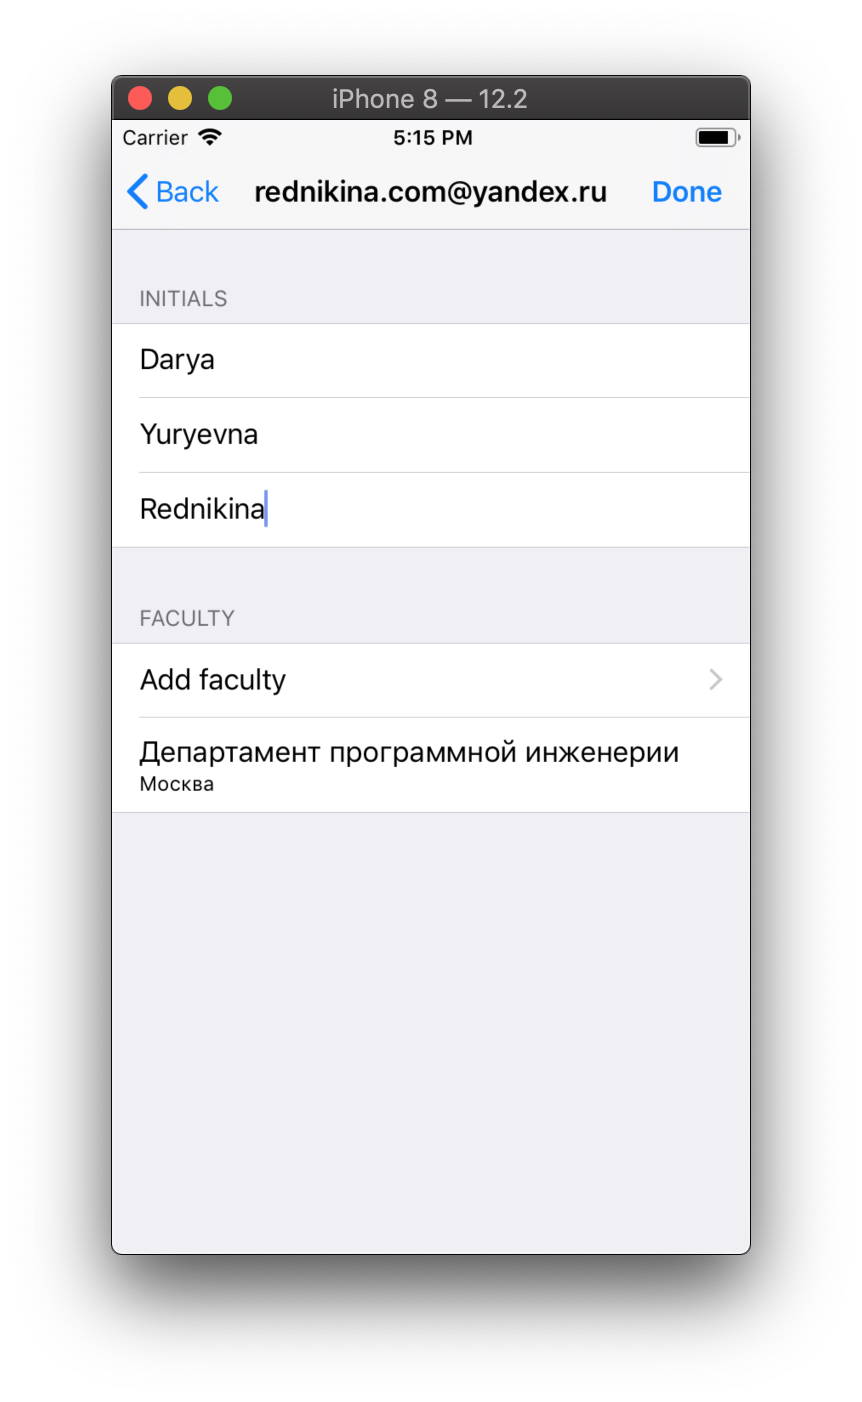
\includegraphics[width=\linewidth]{../includes/pmi/r2.png}
		\end{subfigure}
		\begin{subfigure}[b]{0.3\linewidth}
			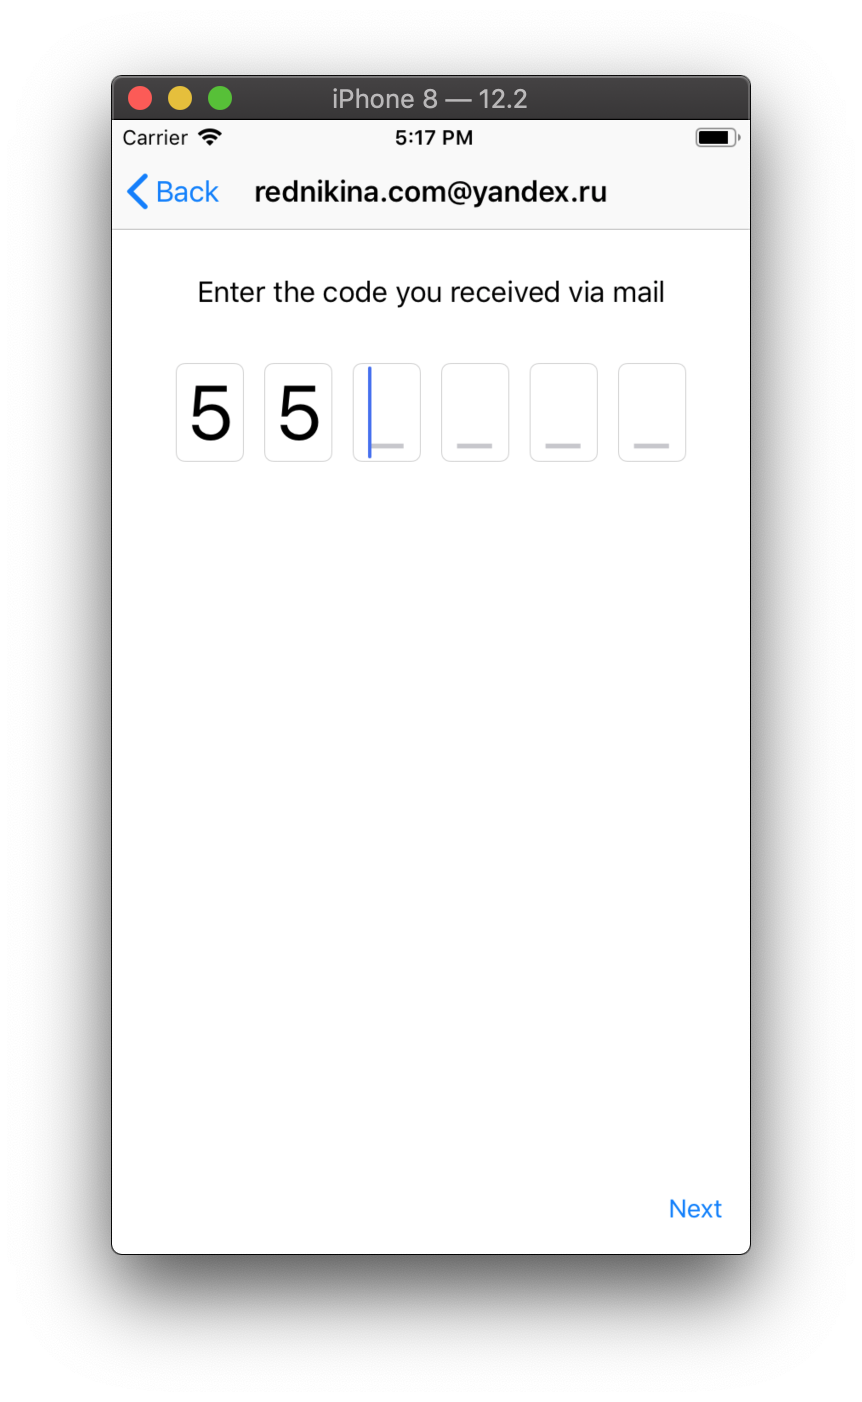
\includegraphics[width=\linewidth]{../includes/pmi/code.png}
		\end{subfigure}
		\caption{\label{pic: register}Регистрация клиента в социальной сети}
	\end{figure}
	\subsubsection{Вход в учетную запись}
	Процесс входа уже зарегистрированного пользователя в собственную учетную запись:
	\begin{enumerate}
		\item Ввод email -- происходит отправка запрос на сервер для валидации данных
		\item При успешной валидации почты на сервере, происходит получение письма на введенную почту с кодом подтверждения 
		\item Клиент вводит полученный код в специальное поле -- при успешной валидации кода клиент входит в приложение
	\end{enumerate}
	\begin{figure}[h!]
		\centering
		\begin{subfigure}[b]{0.3\linewidth}
			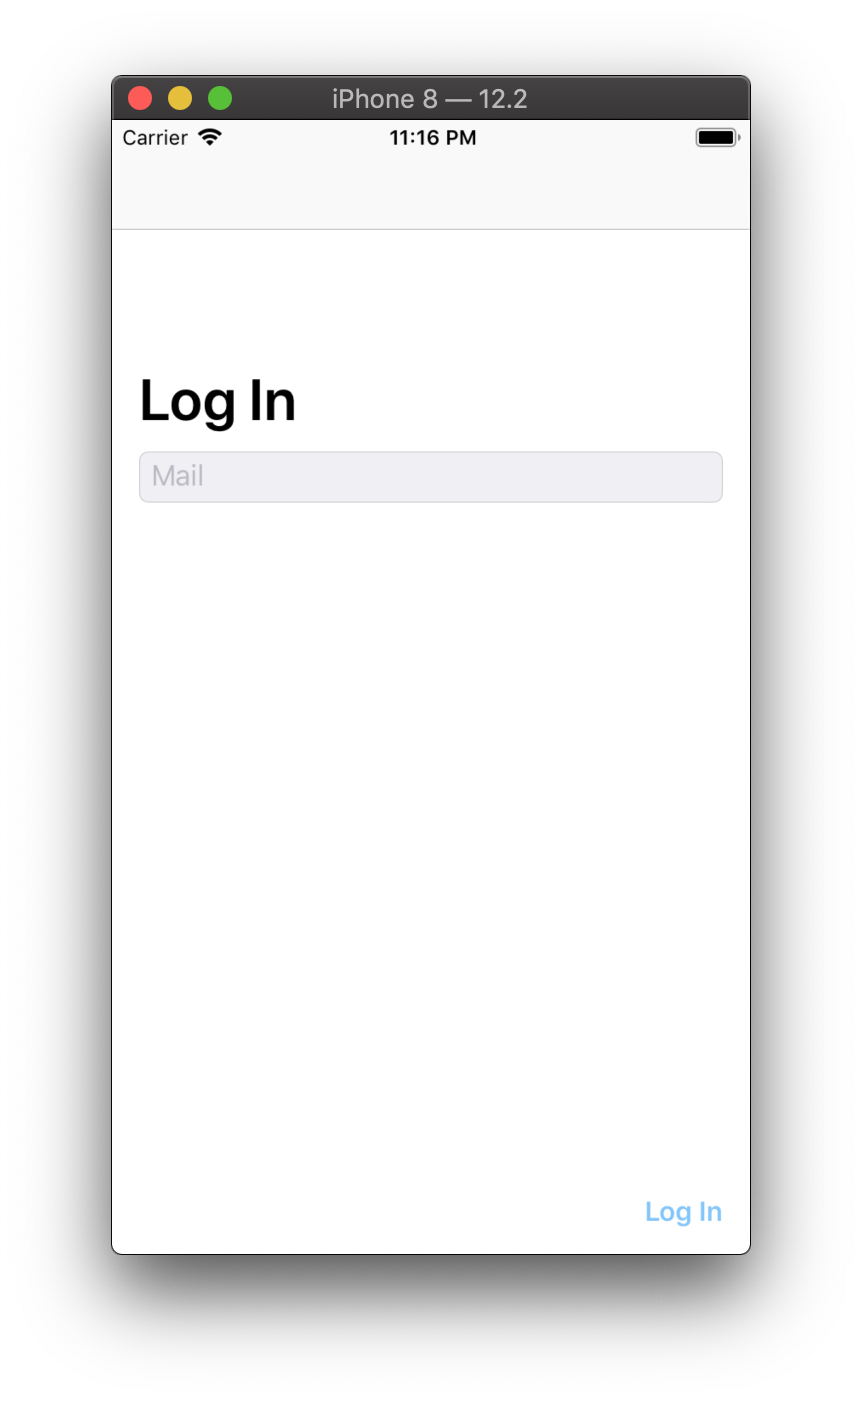
\includegraphics[width=\linewidth]{../includes/pmi/login.png}
		\end{subfigure}
		\begin{subfigure}[b]{0.3\linewidth}
			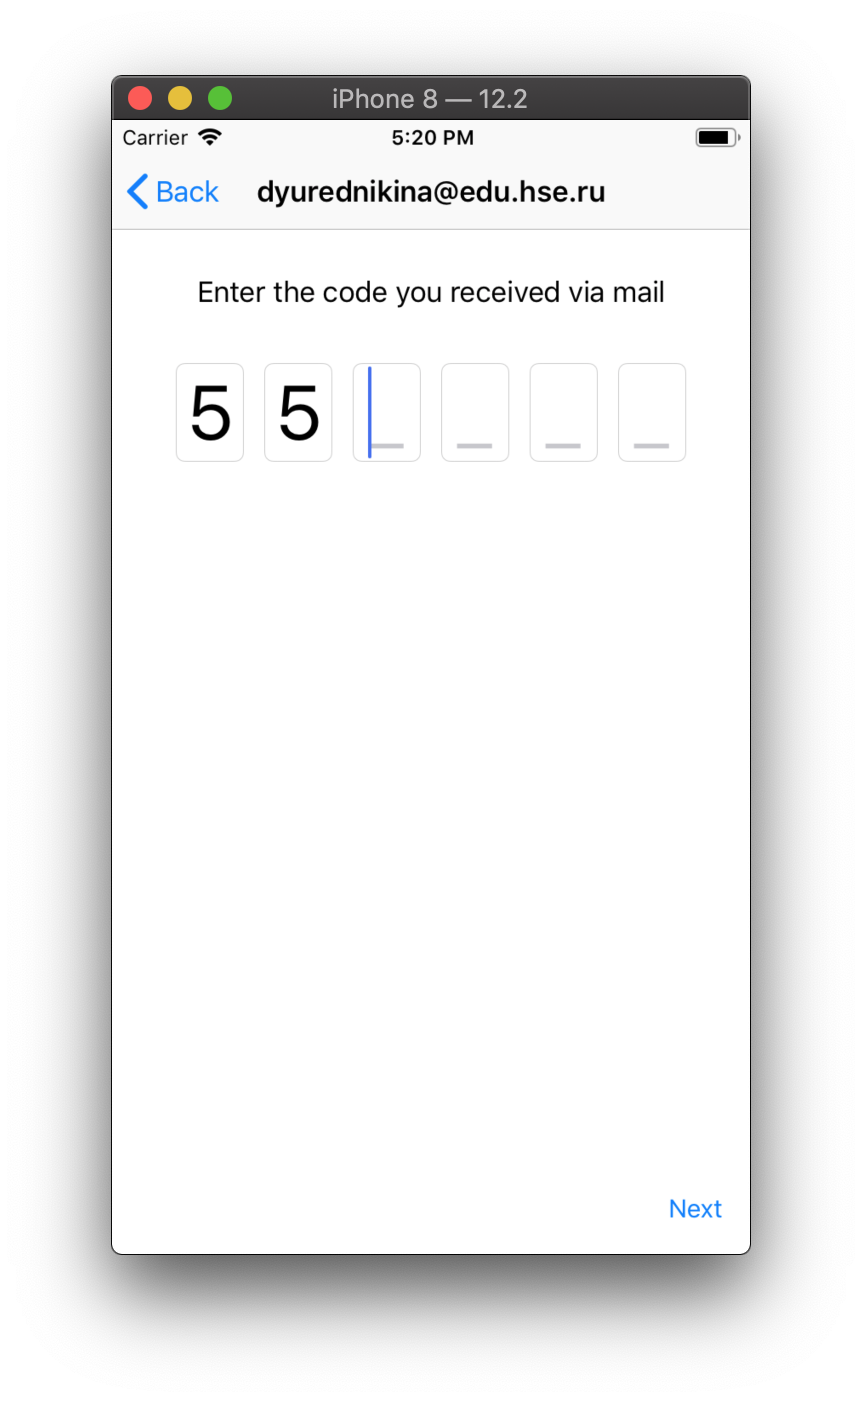
\includegraphics[width=\linewidth]{../includes/pmi/code1.png}
		\end{subfigure}
		\begin{subfigure}[b]{0.3\linewidth}
			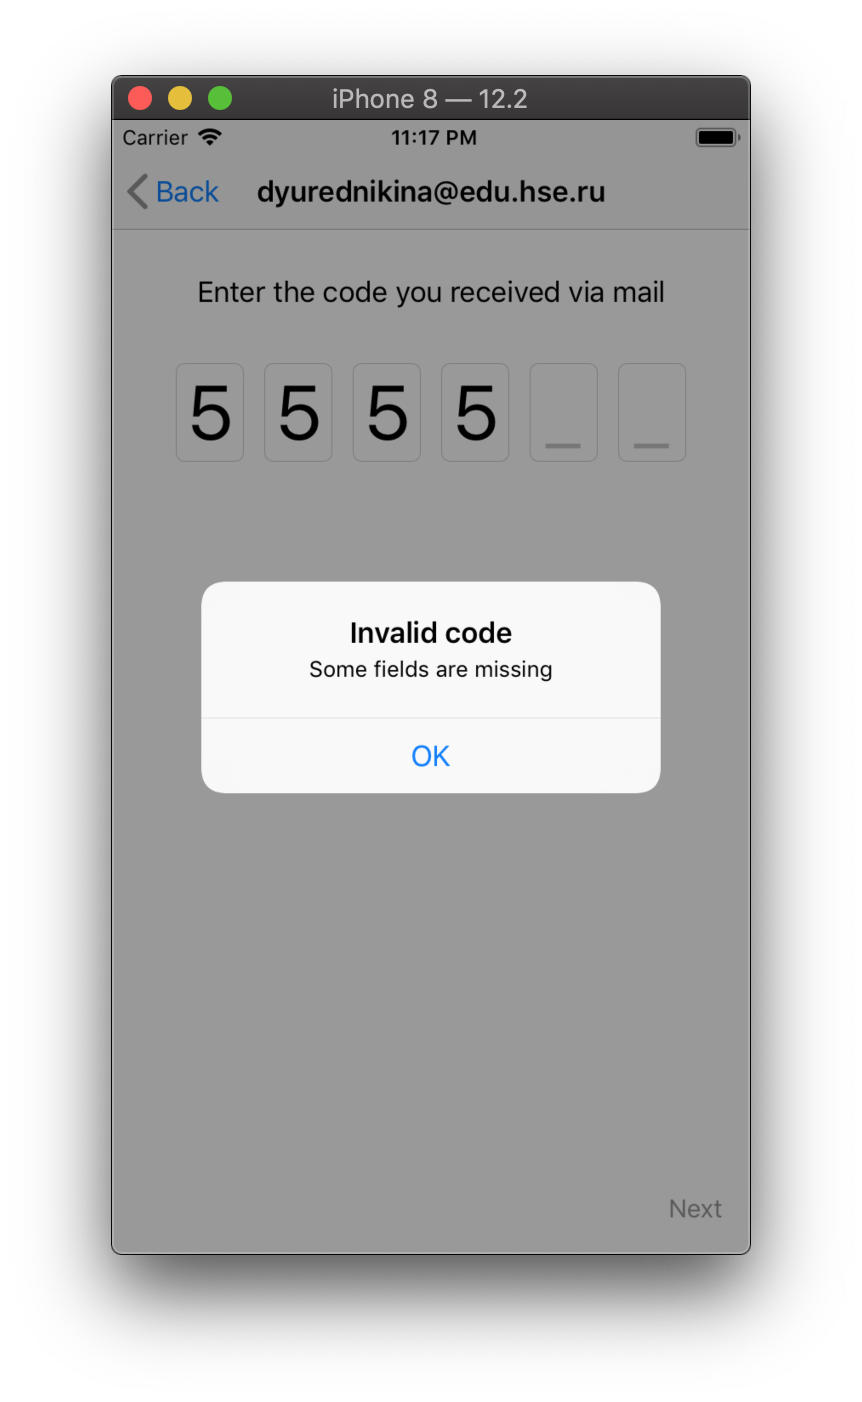
\includegraphics[width=\linewidth]{../includes/pmi/invalidcode.png}
		\end{subfigure}
		\caption{\label{pic: auto} Авторизация клиента в социальной сети}
	\end{figure}
	\clearpage
	\subsubsection{Просмотр ленты новостей}
	При входе в приложение пользователь видит общую ленту всех новостей \textit{General}. Клиент может с помощью строки поиска найти посты по интересущей его тематике (см. рис \ref{sub: search}, \ref{sub: ios}), а также просто просматривать ленту новостей, открывать полное содержание поста в ленте (см. рис \ref{sub: fullpost}) при нажатии на текст поста, а также переходить на профили пользователей -- авторов постов, при нажатии на их имя.
	
	\begin{figure}[h!]
		\centering
		\begin{subfigure}[b]{0.3\linewidth}
			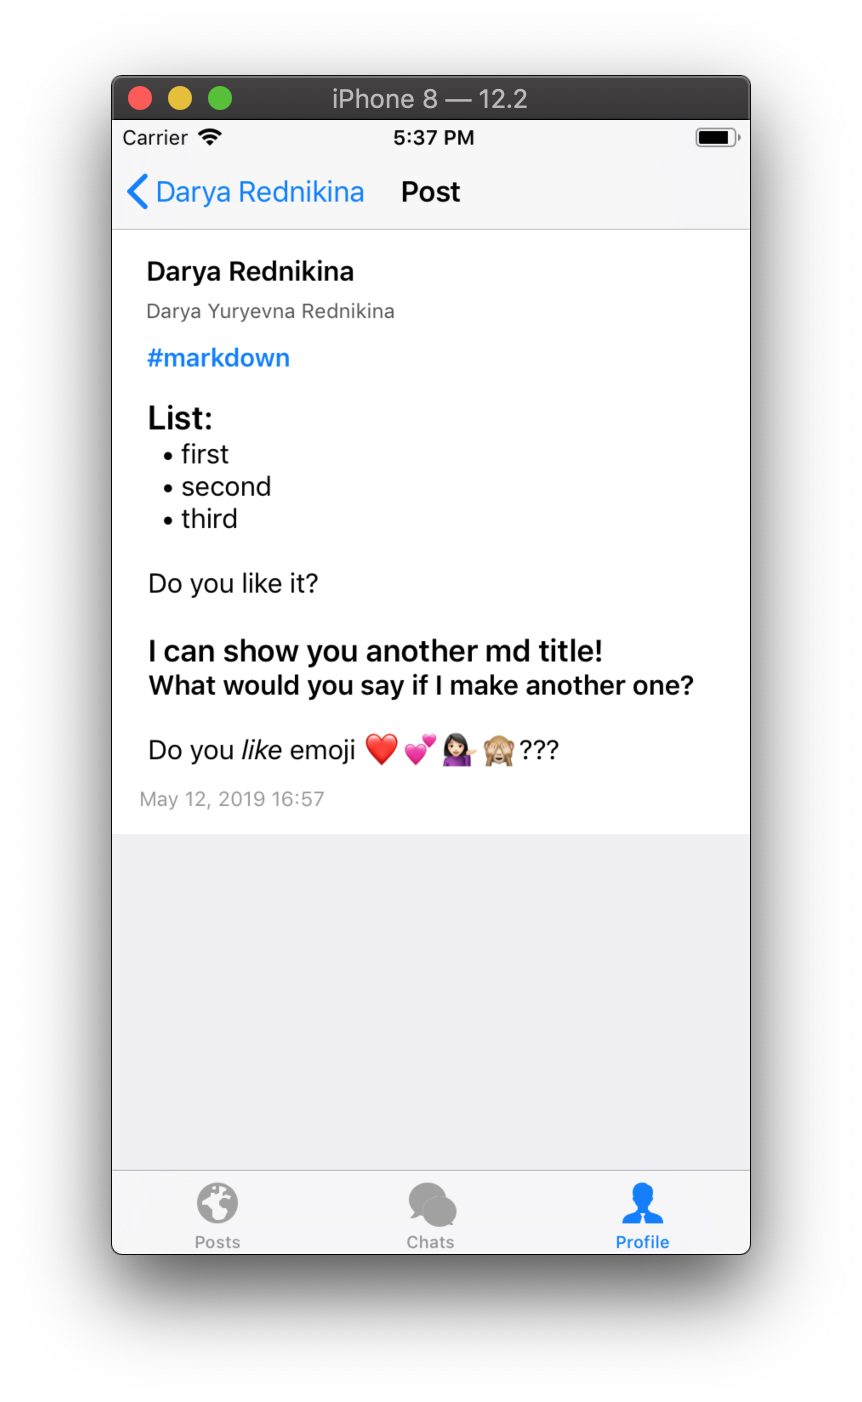
\includegraphics[width=\linewidth]{../includes/pmi/profile_fullpost.png}
			\caption{\label{sub: fullpost}Просмотр поста}
		\end{subfigure}
		\begin{subfigure}[b]{0.3\linewidth}
			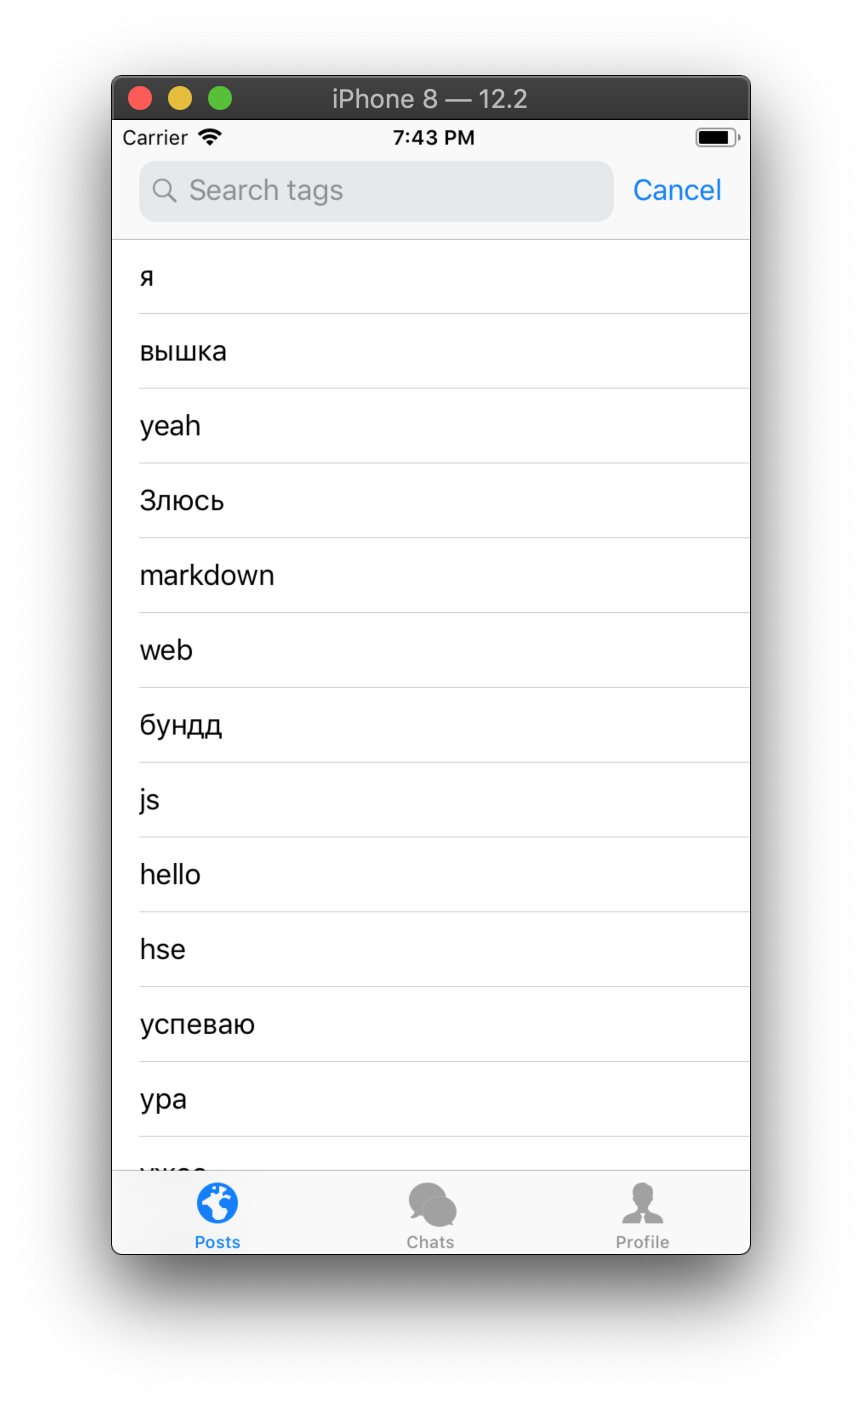
\includegraphics[width=\linewidth]{../includes/pmi/search.png}
			\caption{\label{sub: search}Поиск}
		\end{subfigure}
		\begin{subfigure}[b]{0.3\linewidth}
			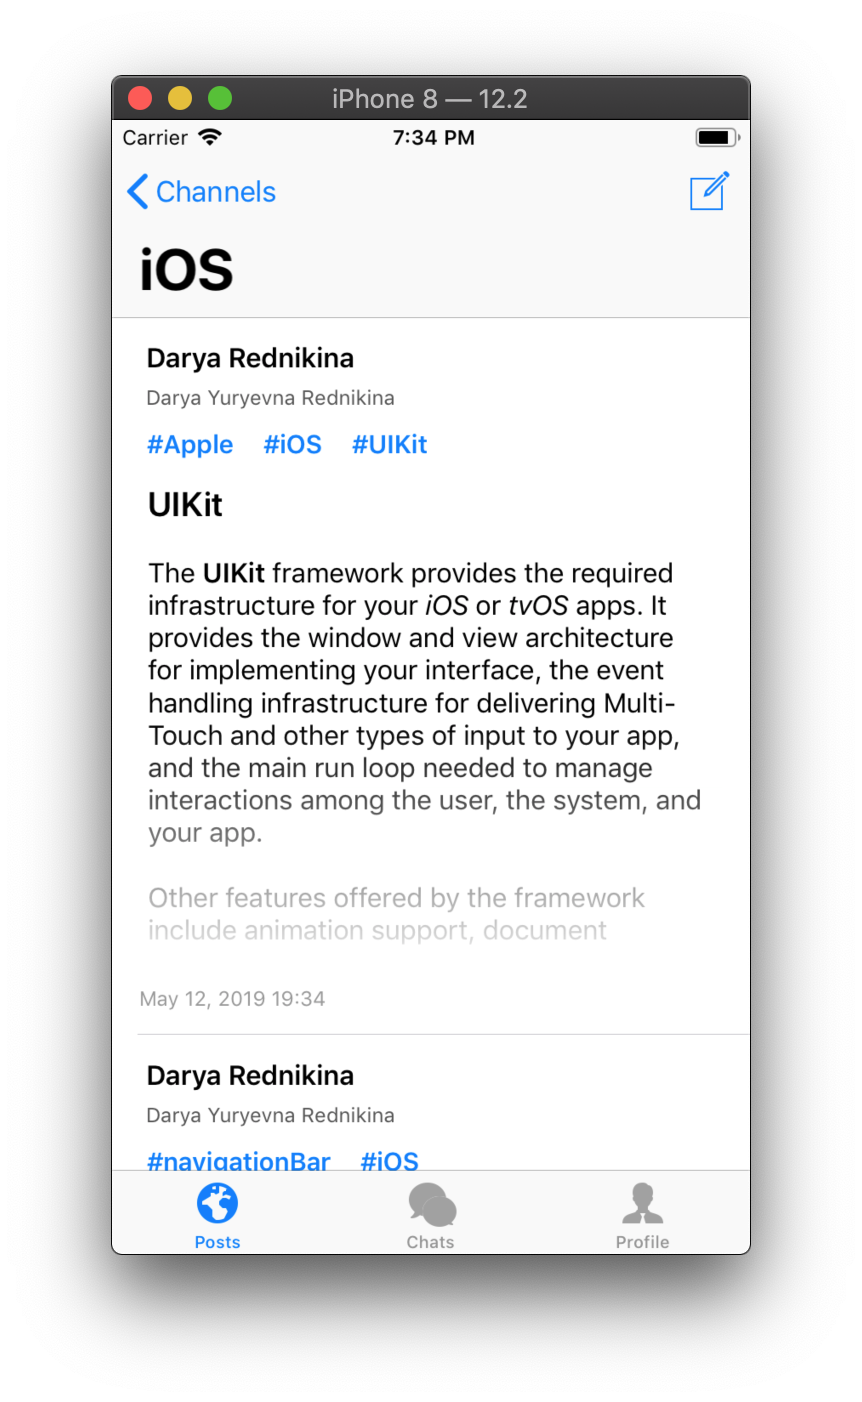
\includegraphics[width=\linewidth]{../includes/pmi/ios_channel.png}
			\caption{\label{sub: ios}Интересующая тематика}
		\end{subfigure}
		\caption{\label{pic: n}Просмотр ленты}
	\end{figure}
	\clearpage
	\subsubsection{Написание и публикация поста}
	Находясь в канале/в общей ленте, клиент имеет возможность написать пост, нажав кнопку в правом верхнем углу. При открытии окна для написания поста пользователь может написать текст а также добавить хэштеги к посту (см. рис \ref{pic: write}). Публикация поста происходит при нажатии кнопки \textit{Publish}, кнопка \textit{Cancel} предлагает удалить написанный текст или сохранить как черновик для следующего открытия окна для написания поста (cм. рис \ref{pic: draft}).
	
	\begin{figure}[h!]
		\centering
		\begin{subfigure}[b]{0.3\linewidth}
			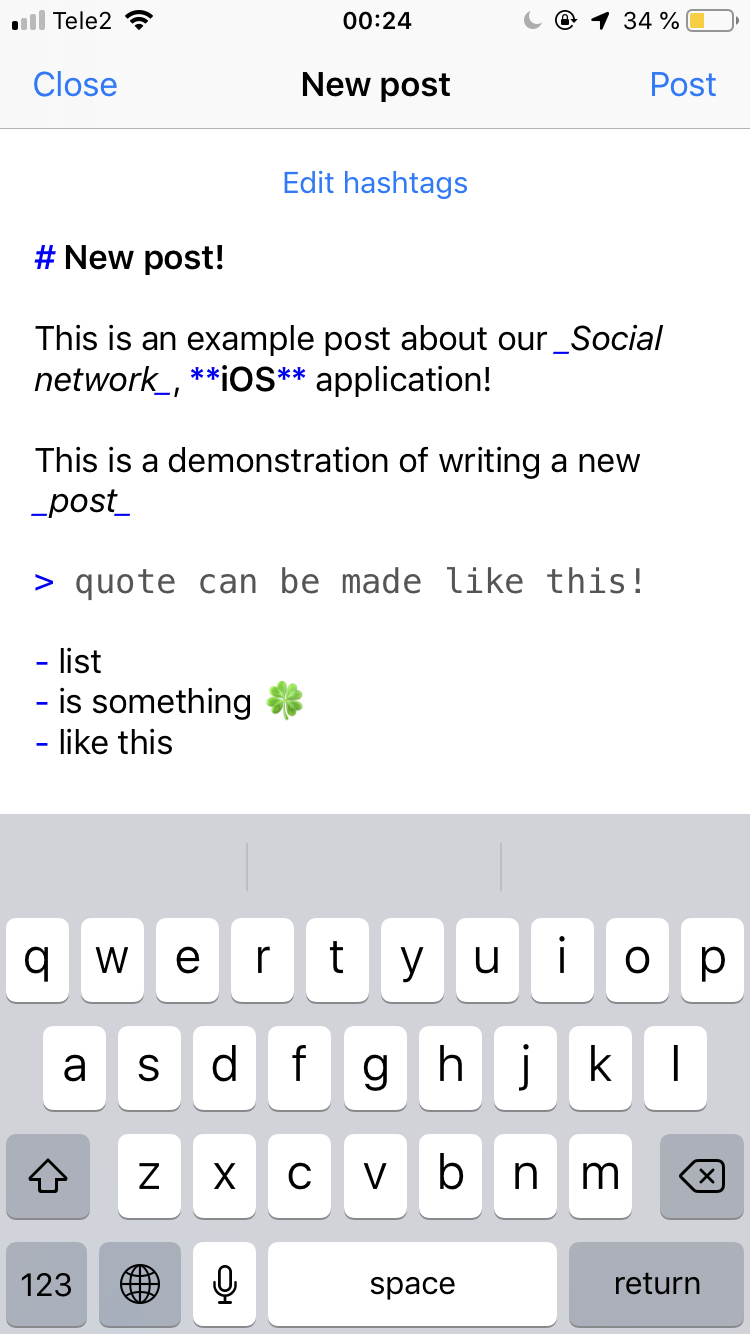
\includegraphics[width=\linewidth]{../includes/ro/newpost.png}
			\caption{\label{pic: write}Написание поста}
		\end{subfigure}
		\begin{subfigure}[b]{0.3\linewidth}
			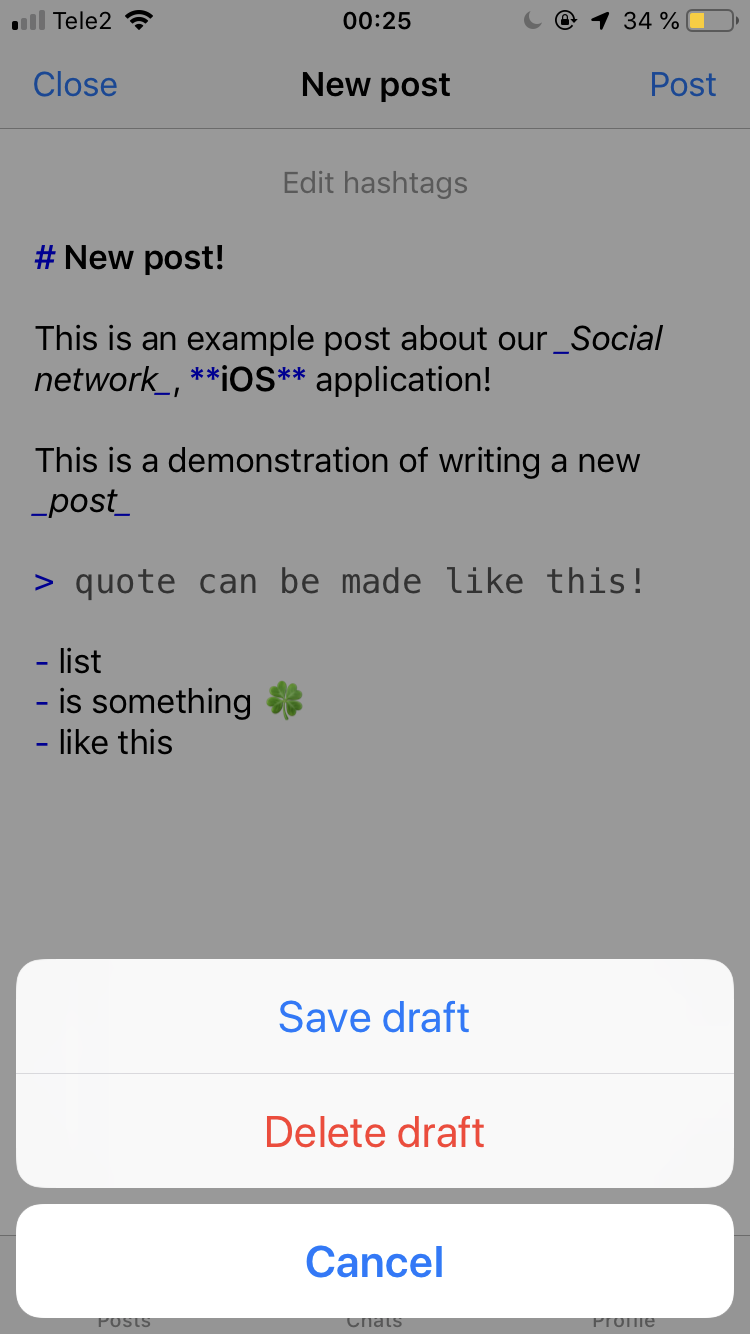
\includegraphics[width=\linewidth]{../includes/ro/draft.png}
			\caption{\label{pic: draft}Черновик}
		\end{subfigure}
		\begin{subfigure}[b]{0.3\linewidth}
			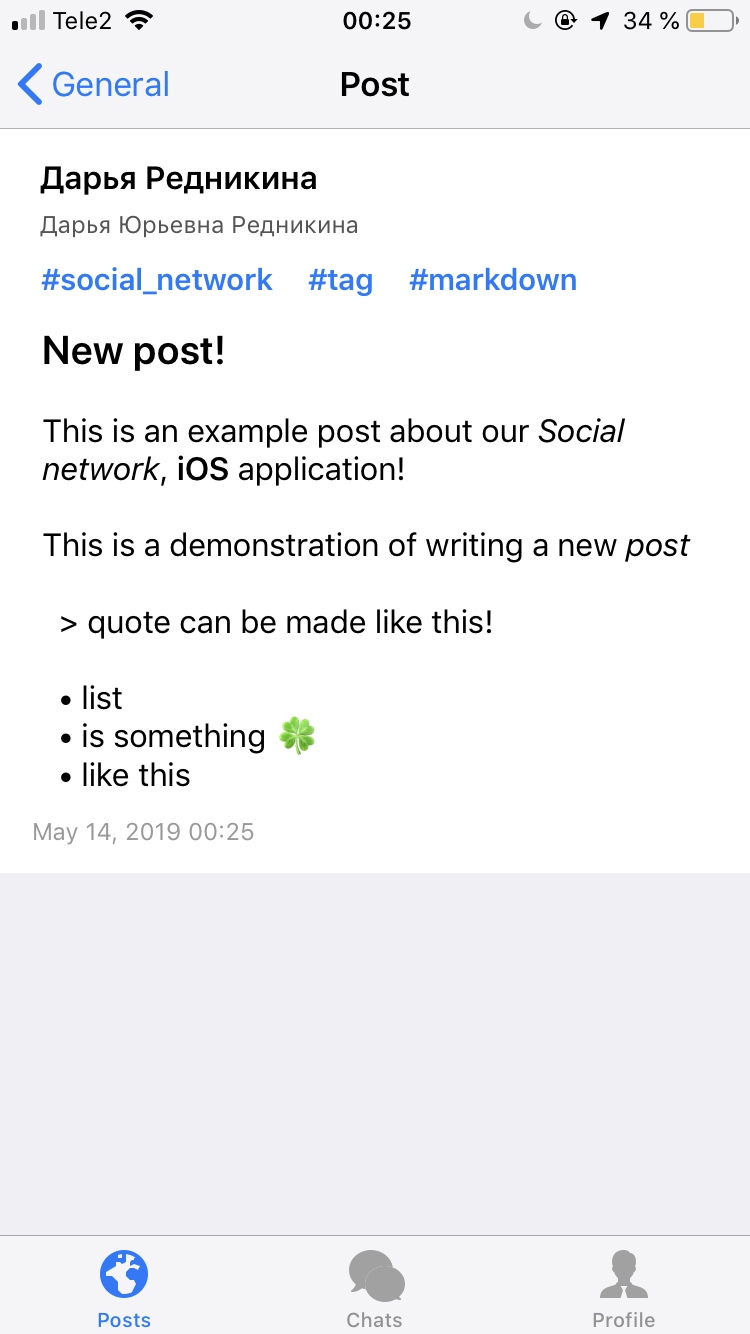
\includegraphics[width=\linewidth]{../includes/ro/display.png}
			\caption{\label{pic: display}Пост в ленте}
		\end{subfigure}
		\caption{\label{pic: writenewpost}Написание и публикация поста}
	\end{figure}
 	\clearpage
	\subsubsection{Просмотр каналов}
	Находясь в канале/в общей ленте, клиент имеет возможность по свайпу вправо (или при нажатии кнопки в левом верхнем углу \textit{Channels}) перейти в полный список каналов (см. рис ). Для просмотра содержимого канала клиенту надо нажать на интересущую его ячейку в списке.
	\begin{figure}[h!]
		\centering
		\begin{subfigure}[b]{0.3\linewidth}
			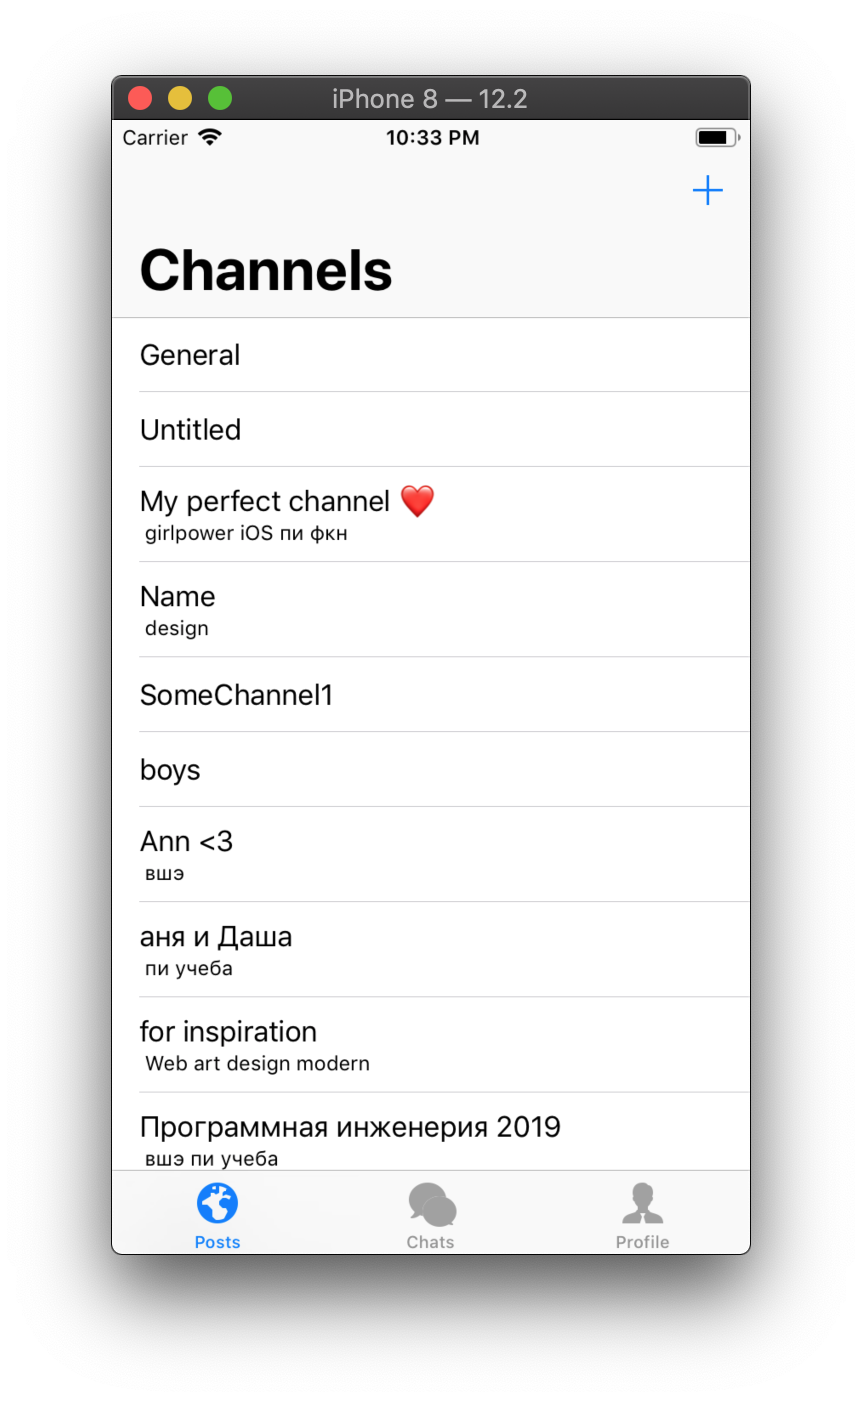
\includegraphics[width=\linewidth]{../includes/pmi/channel_list.png}
		\end{subfigure}
		\begin{subfigure}[b]{0.3\linewidth}
			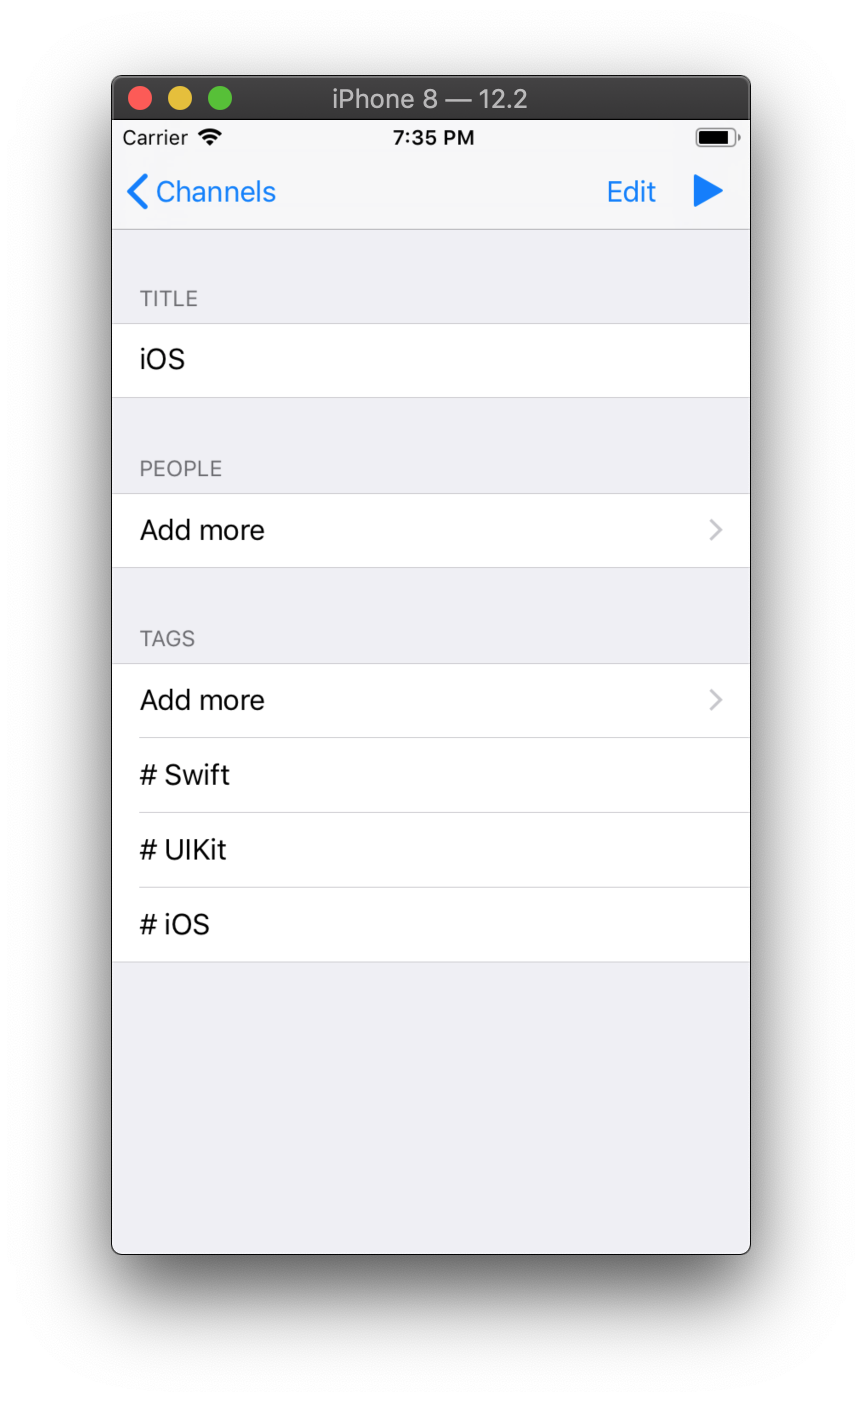
\includegraphics[width=\linewidth]{../includes/pmi/ios_channel_what.png}
		\end{subfigure}
		\begin{subfigure}[b]{0.3\linewidth}
			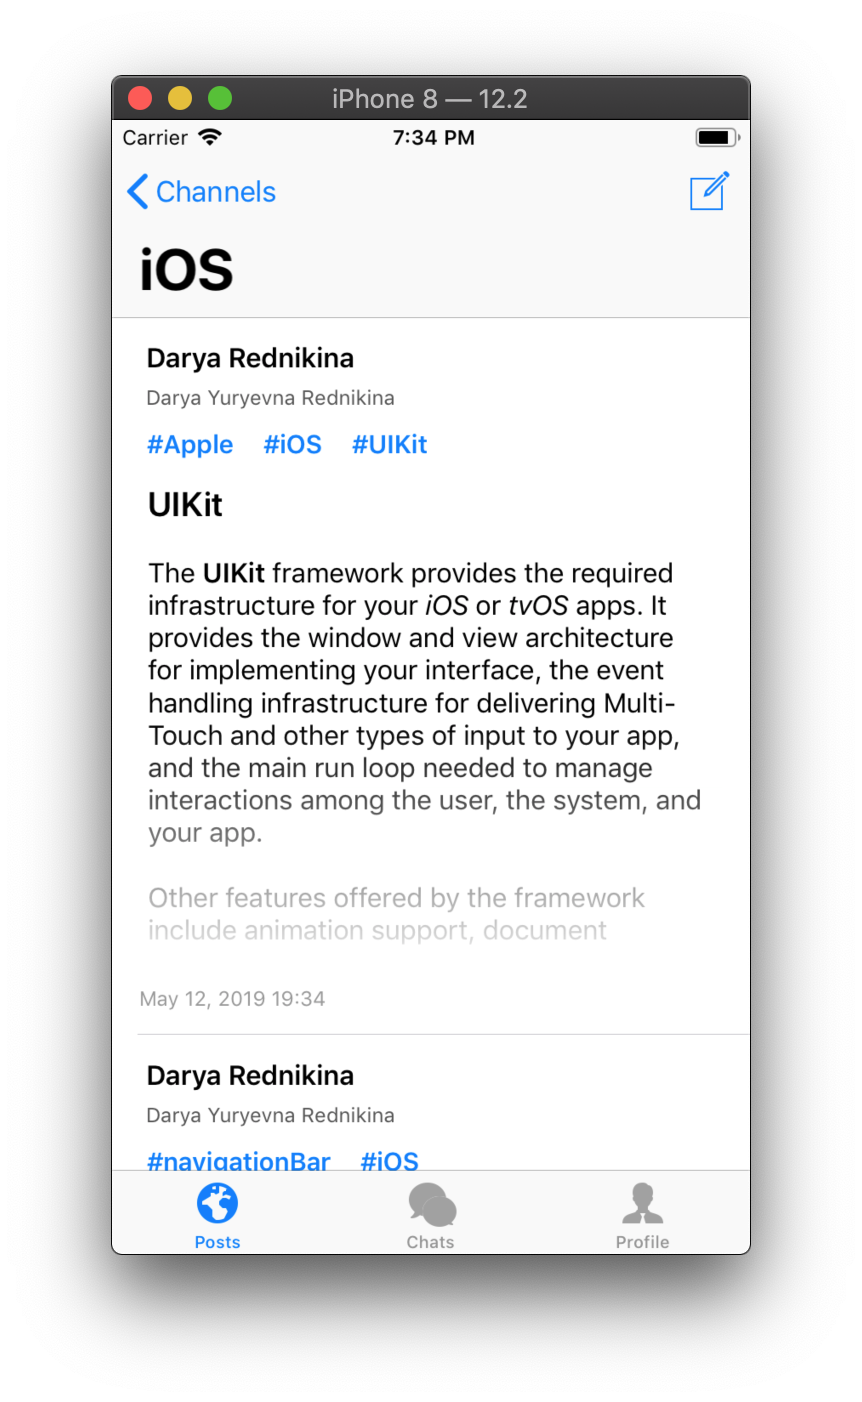
\includegraphics[width=\linewidth]{../includes/pmi/ios_channel.png}
		\end{subfigure}
		\caption{Педпросмотр и просмотр канала}
	\end{figure}
	\clearpage
	\subsubsection{Создание и редактирование каналов}
	Находясь в полном списке каналов, клиент имеет возможность создать канал по нажатию на кнопку <<+>> в правом верхнем углу (см. рис ). При нажатии открывается окно для редактирование содержимого пока что пустого канала (см. рис ): можно отредактировать название нажав на ячейку в первой секции, можно отредактировать множество хэштегов и людей, входящих в канал, нажав на ячейку \textit{Add more} в каждой секции (<<People>>, <<Hashtags>>) соответственно (см. рис ). Также можно удалить элементы из списков при нажатии кнопки \textit{Edit} в правом верхнем углу и выборе соответствующих элементов для удаления (см. рис). 
	\begin{figure}[h!]
		\centering
		\begin{subfigure}[b]{0.3\linewidth}
			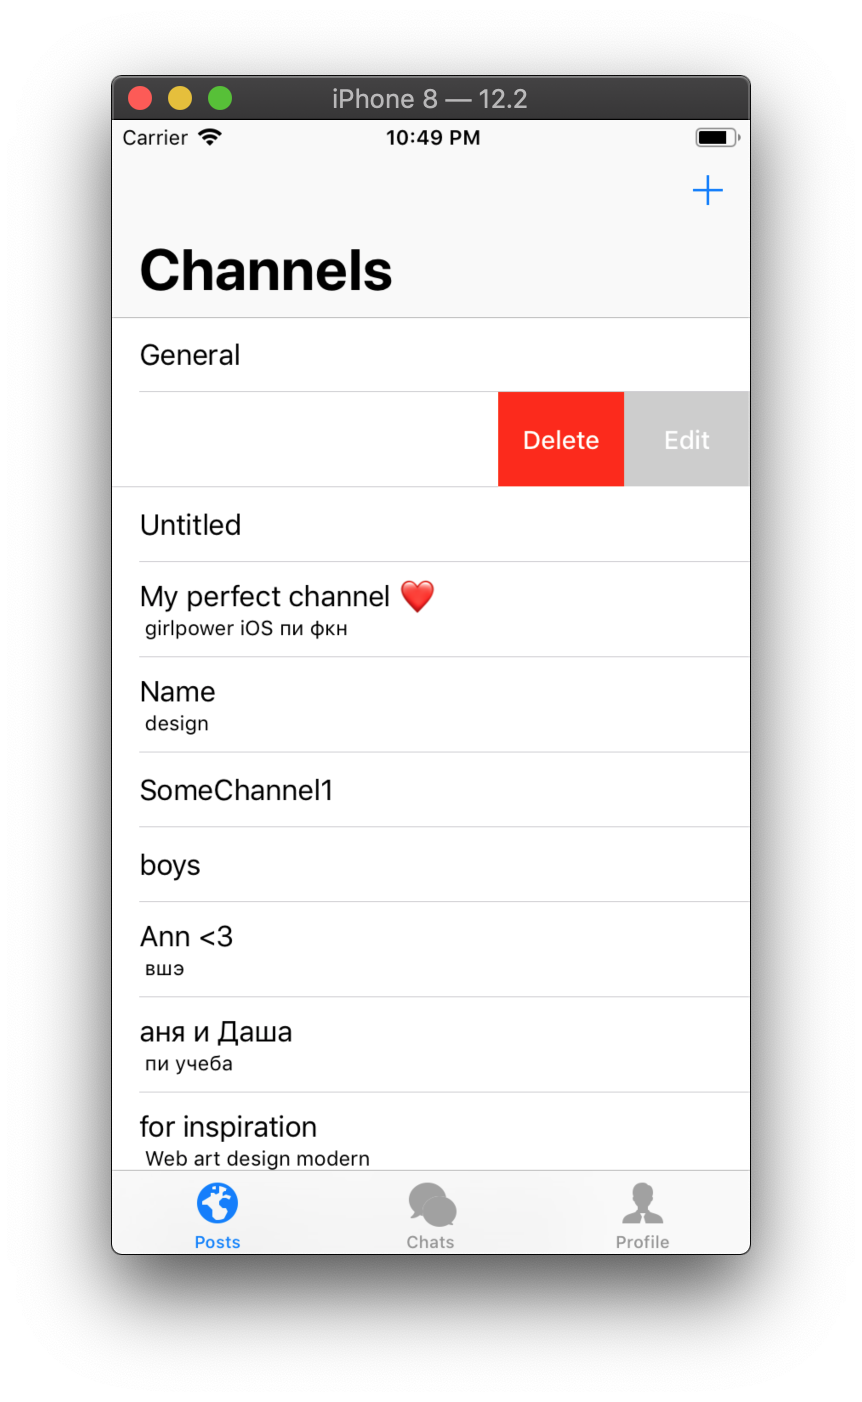
\includegraphics[width=\linewidth]{../includes/pmi/edit.png}
		\end{subfigure}
		\begin{subfigure}[b]{0.3\linewidth}
			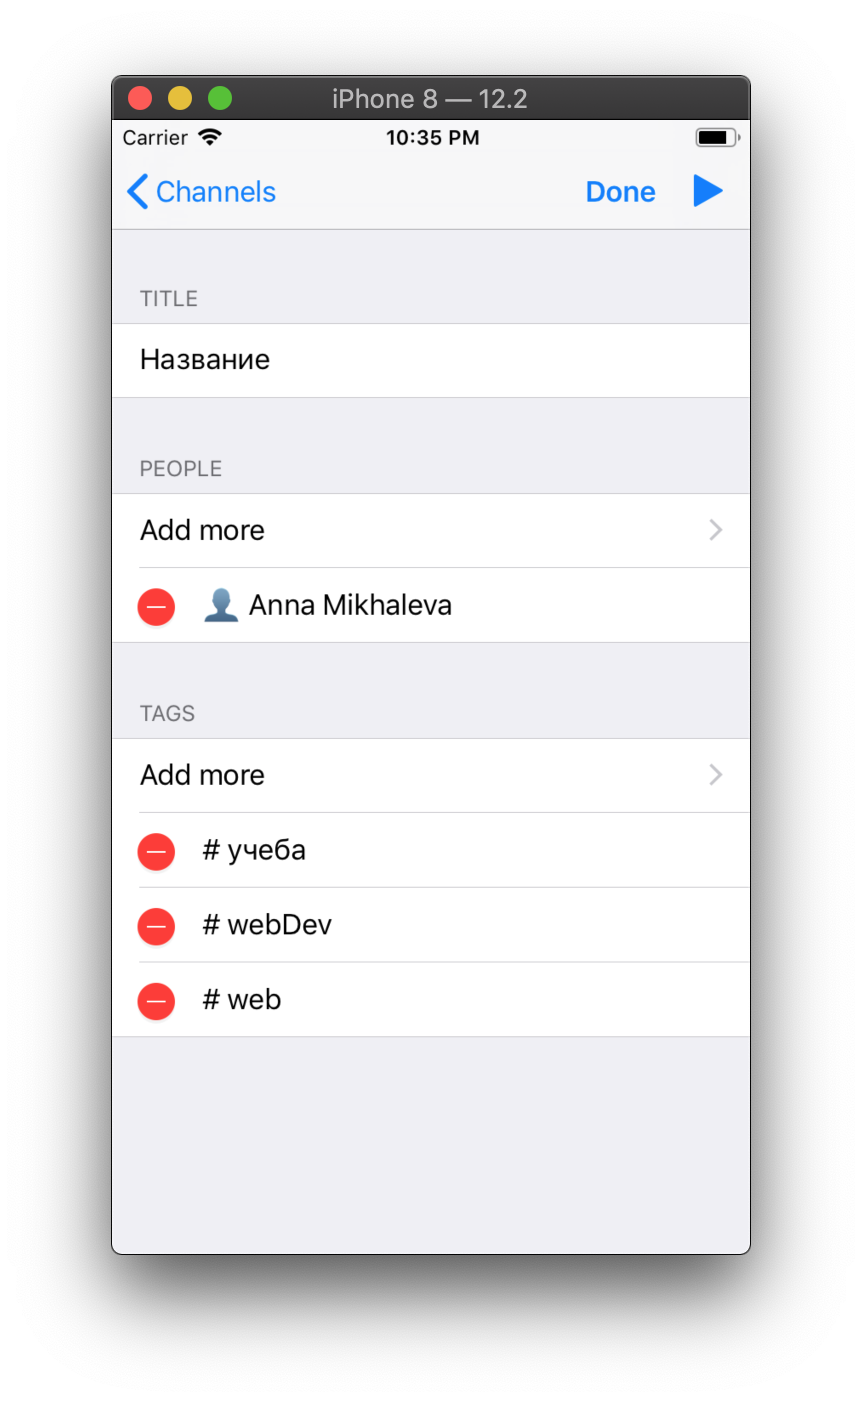
\includegraphics[width=\linewidth]{../includes/pmi/edit_button_channel.png}
		\end{subfigure}
		\begin{subfigure}[b]{0.3\linewidth}
			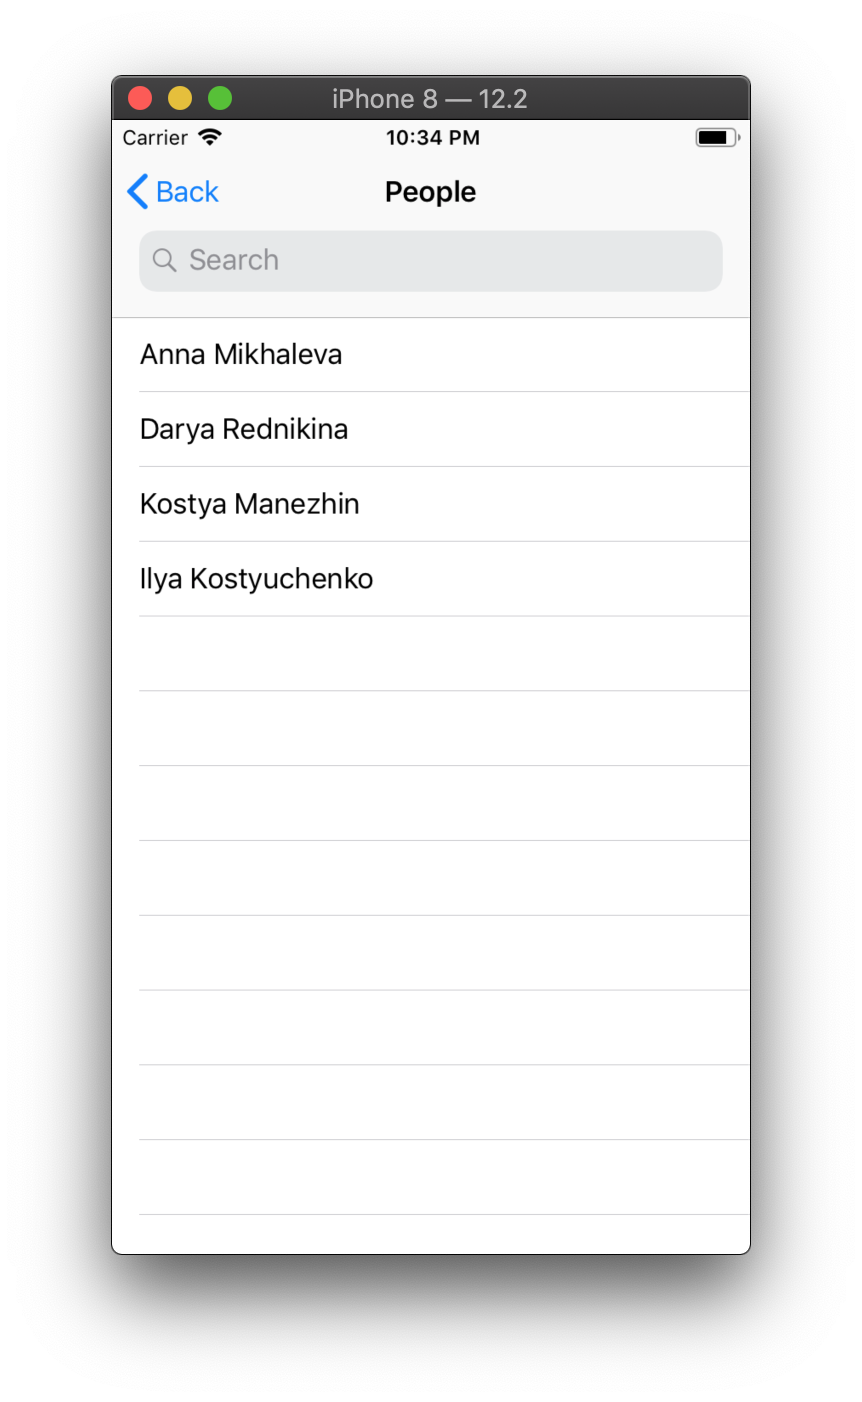
\includegraphics[width=\linewidth]{../includes/pmi/choose_peple.png}
		\end{subfigure}
		\begin{subfigure}[b]{0.3\linewidth}
			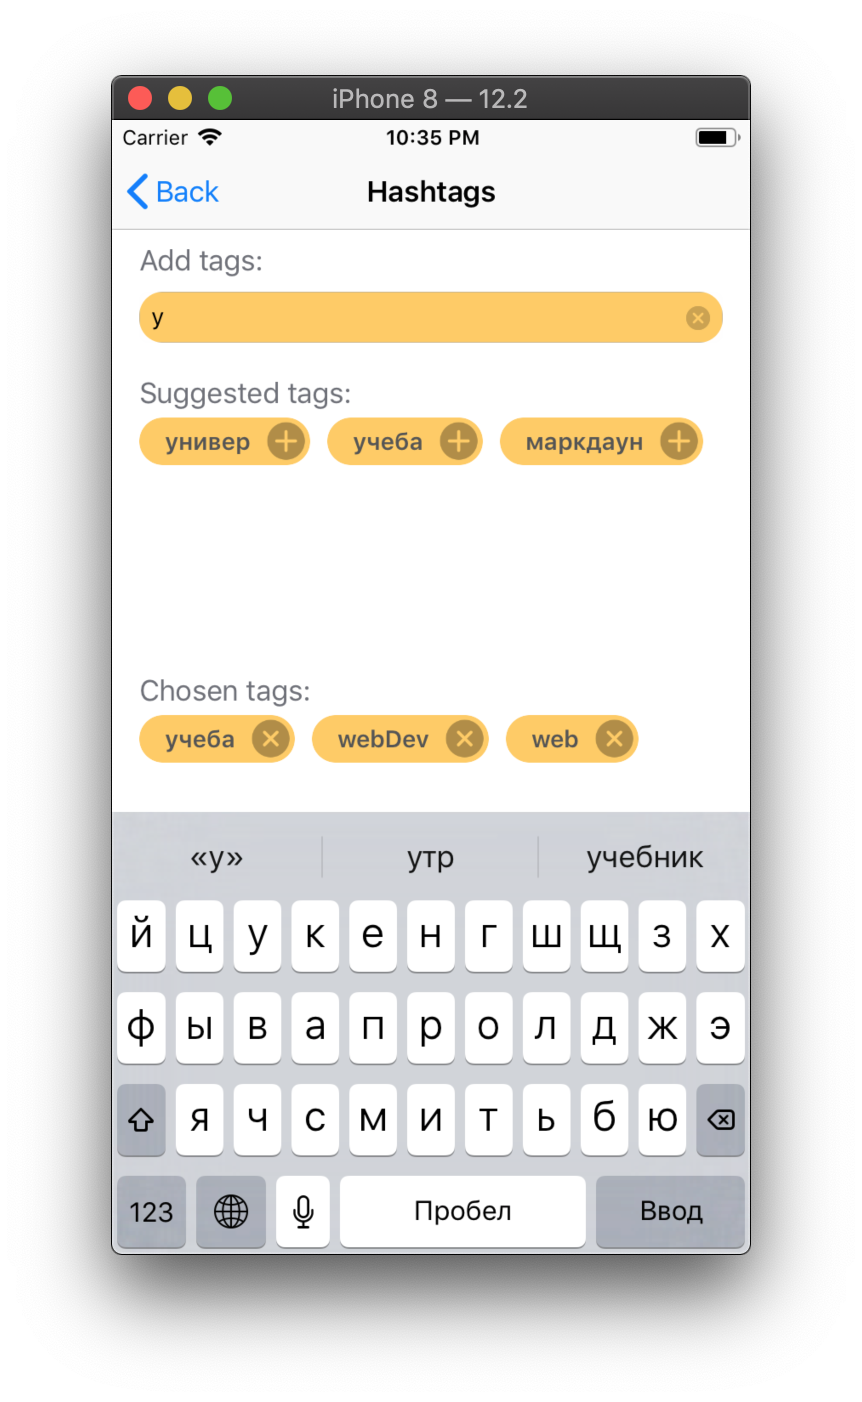
\includegraphics[width=\linewidth]{../includes/pmi/choose_hashtag.png}
		\end{subfigure}
		\begin{subfigure}[b]{0.3\linewidth}
			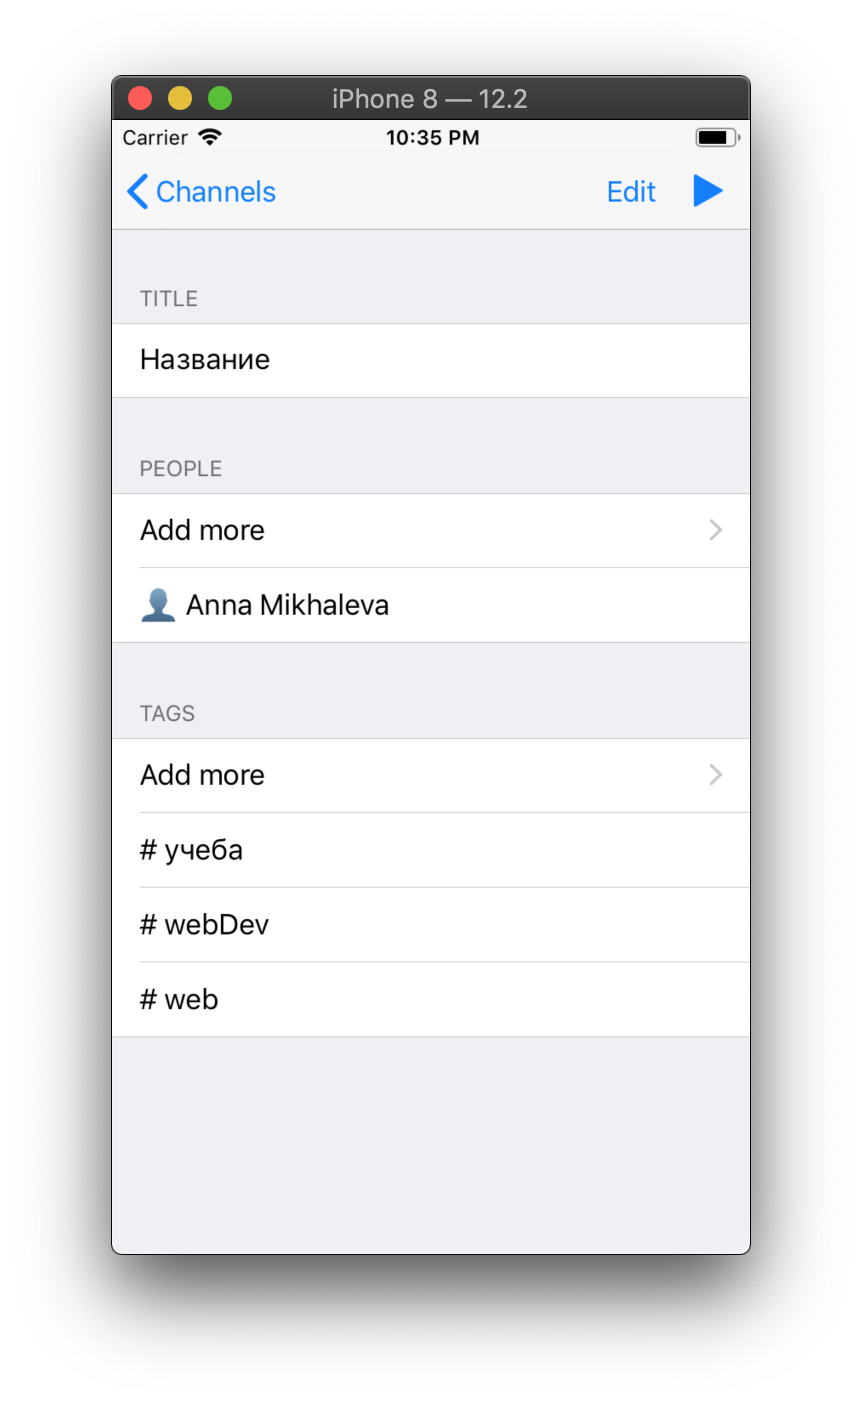
\includegraphics[width=\linewidth]{../includes/pmi/after_editing.png}
		\end{subfigure}
		\caption{\label{pic: editChannl}Редактирование канала}
	\end{figure}
	\clearpage
	\subsubsection{Просмотр сообщений}
	Для просмотра сообщений клиент должен выбрать \textit{Messages} секцию на таббаре (см. рис ). 
		\begin{figure}[h!]
		\centering
		\begin{subfigure}[b]{0.3\linewidth}
			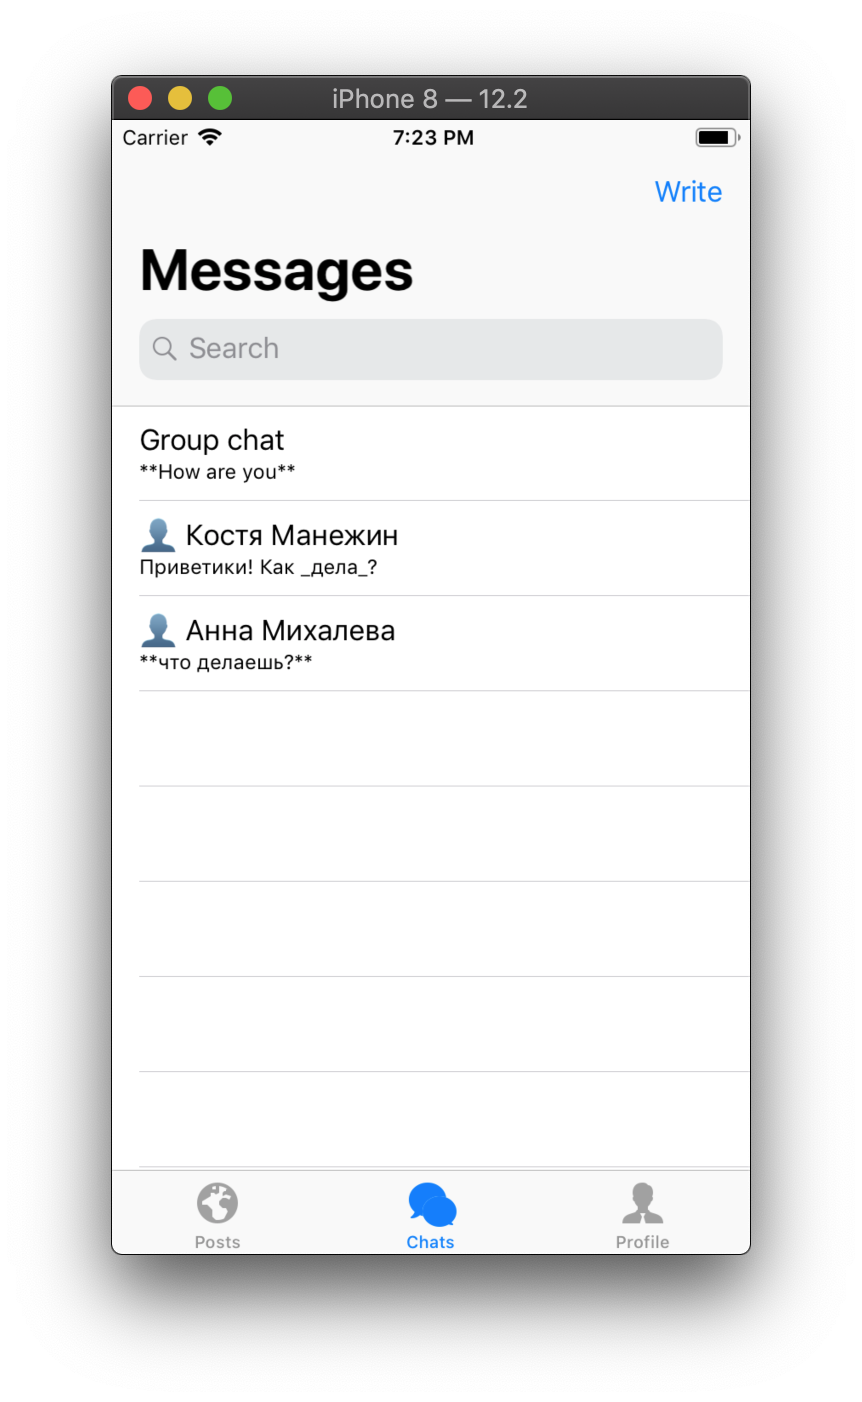
\includegraphics[width=\linewidth]{../includes/pmi/chats.png}
		\end{subfigure}
		\begin{subfigure}[b]{0.3\linewidth}
			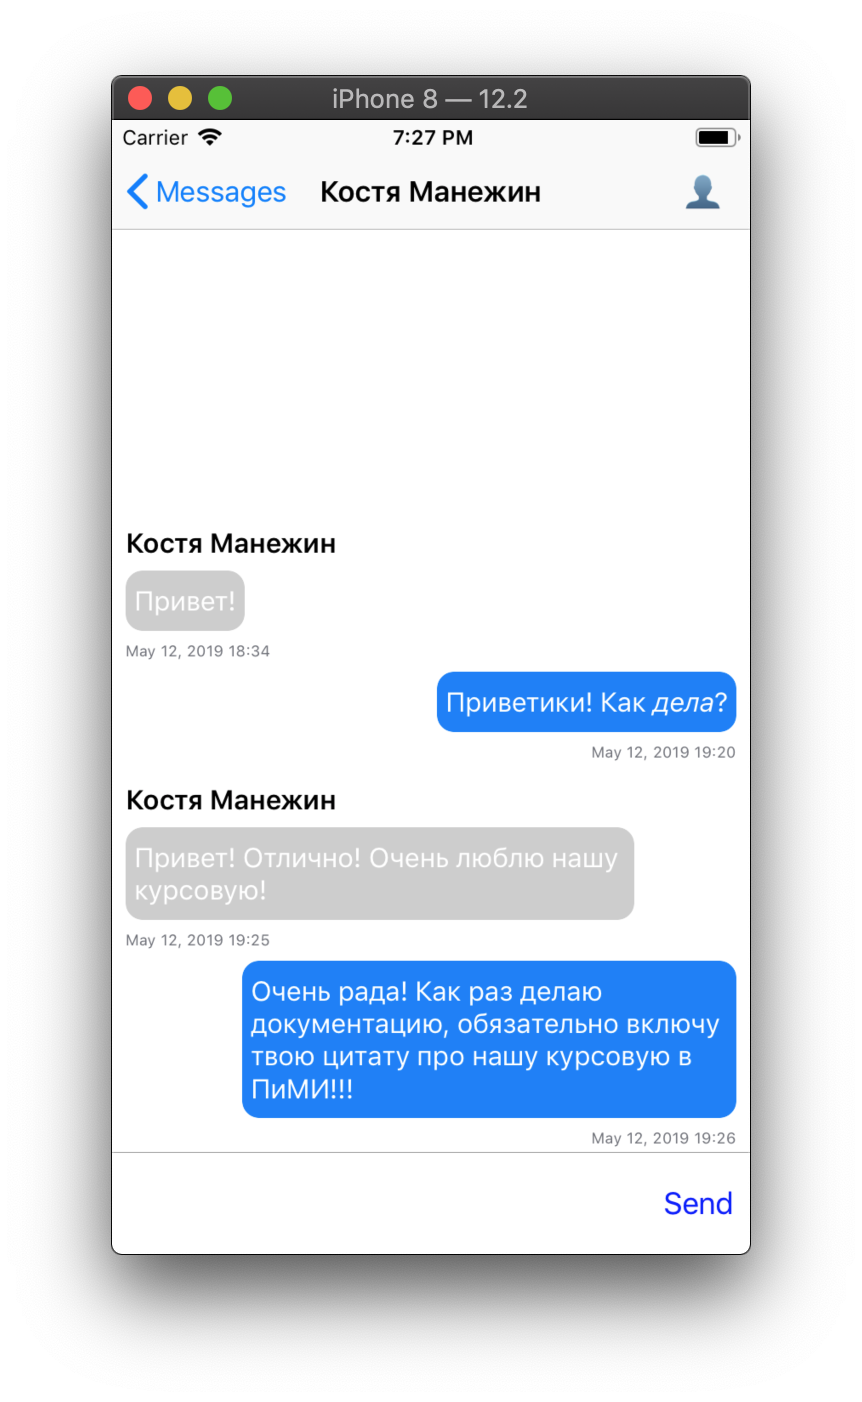
\includegraphics[width=\linewidth]{../includes/pmi/userChat.png}
		\end{subfigure}
		\begin{subfigure}[b]{0.3\linewidth}
			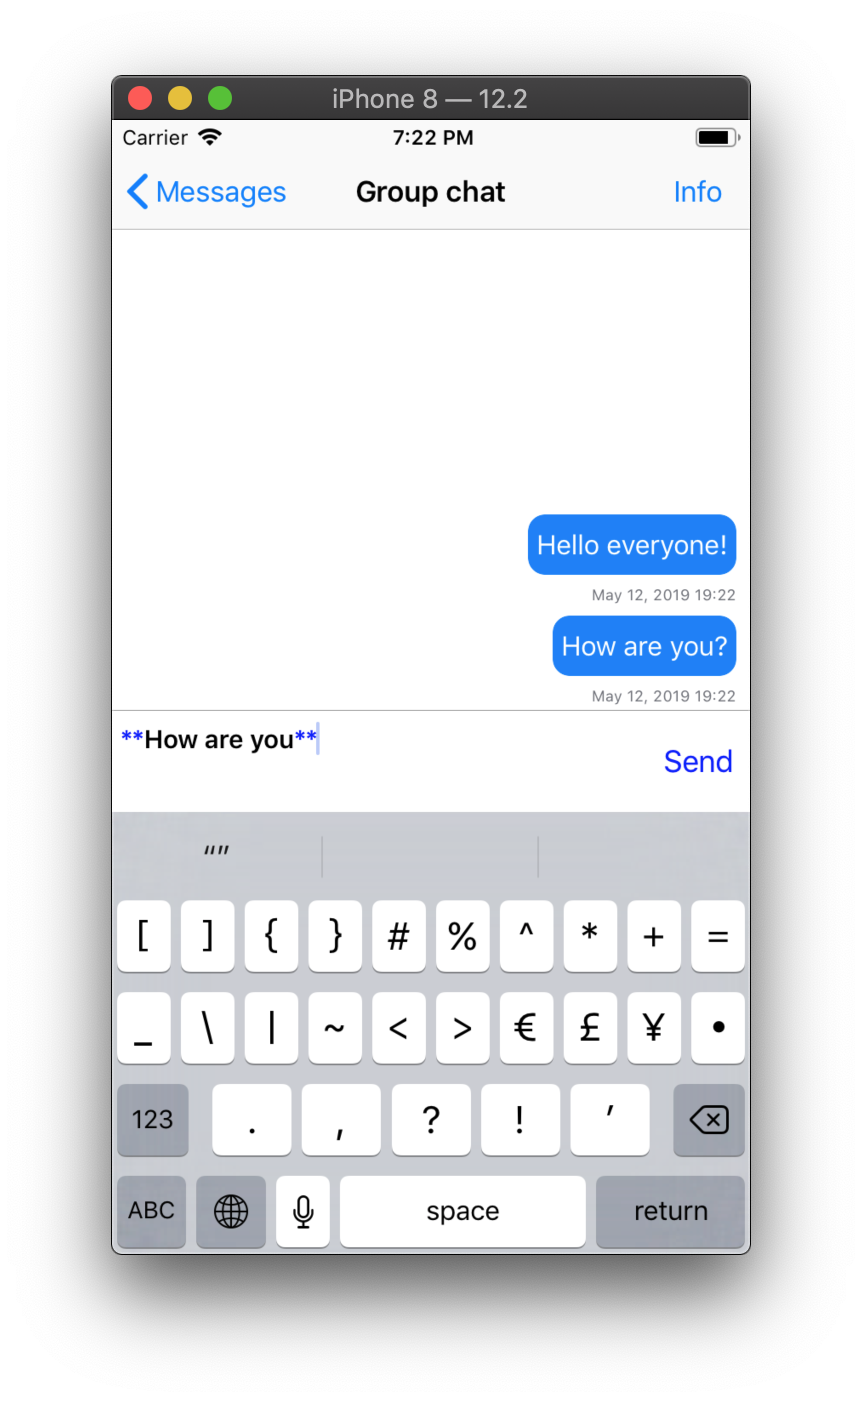
\includegraphics[width=\linewidth]{../includes/pmi/groupChat.png}
		\end{subfigure}
		\caption{\label{pic: chats}Беседы и чаты}
	\end{figure}
\clearpage
	\subsubsection{Создание беседы и администрирование}
	Для создания чата или беседы пользователь должен нажать кнопку \textit{Write} в правом верхнем углу списка диалогов и выбрать людей (2 или больше для создания беседы, 1 -- для чата) (см. рис ). Для просмотра информации (и редактирования при правах администратора) в беседе клиенту надо нажать кнопку \textit{Info} (см. рис). Пользователь, находящийся в беседе, может быть администратором или не иметь прав администратора (см. рис). Пользователь, являющийся администратором, может назначить участников беседы администраторами или отобрать у них это право. Также администратор может менять название чата и добавлять людей при нажатии ячейки \textit{Add people} (см. рис).
	\begin{figure}[h!]
		\centering
		\begin{subfigure}[b]{0.3\linewidth}
			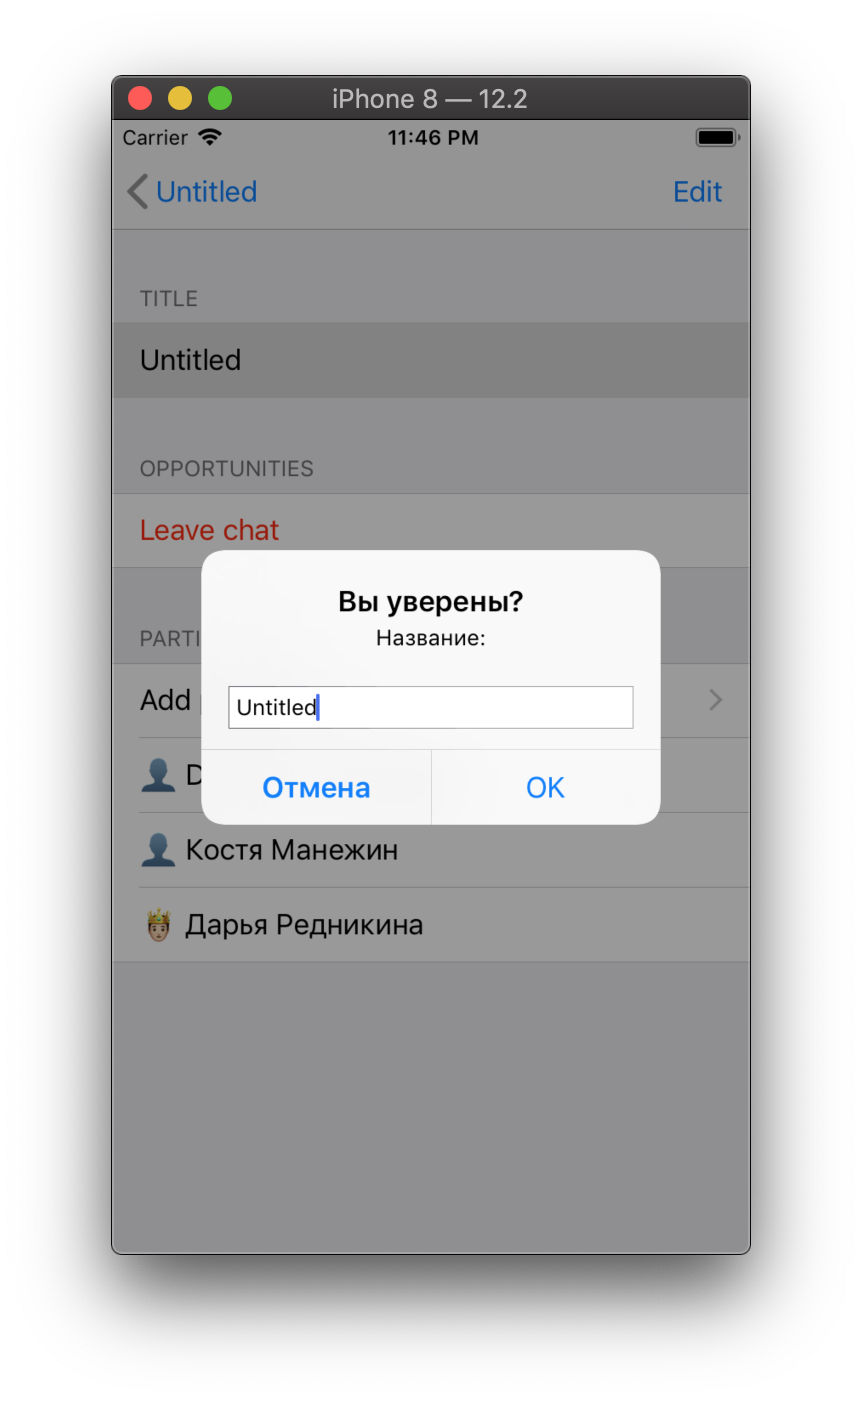
\includegraphics[width=\linewidth]{../includes/pmi/adminName.png}
		\end{subfigure}
		\begin{subfigure}[b]{0.3\linewidth}
			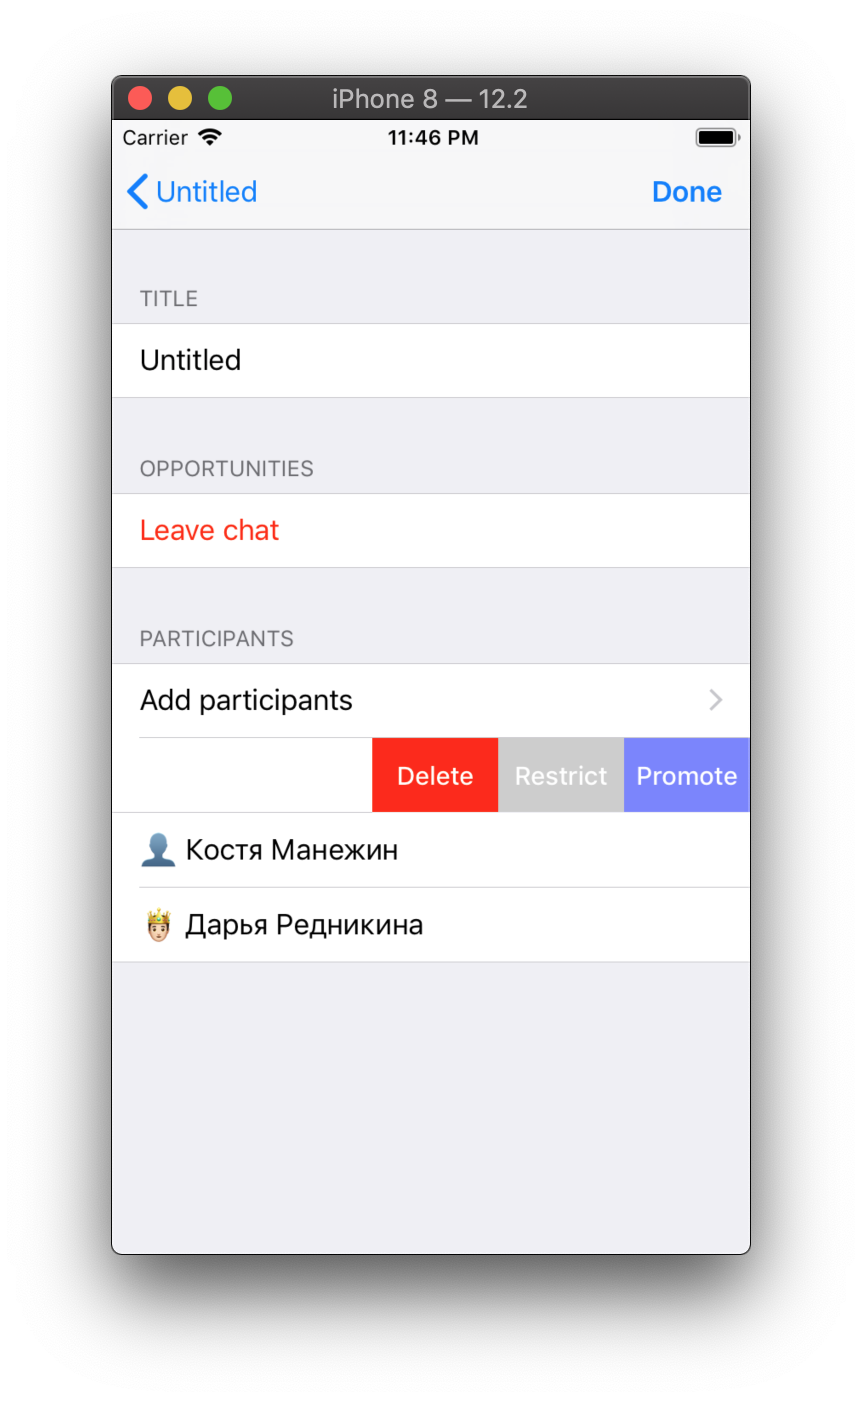
\includegraphics[width=\linewidth]{../includes/pmi/adminChange.png}
		\end{subfigure}
		\caption{\label{pic: admin}Администрирование беседы}
	\end{figure}
\clearpage
	\subsubsection{Просмотр профиля пользователя}
	Для просмотра собственного профиля пользователь должен выбрать \textit{Profile} секцию на таббаре (см. рис \ref{pic: mypr}). На странице пользователя есть возможность просматривать посты, опубликованные пользователем, их полные версии. Также клиент может просмотреть базовую информацию о пользователе выбрав \textit{Basic info} в сегментном контроле (см. рис \ref{pic: bi}). Есть возможность при нажатии справа сверху кнопки \textit{Info} добавить профиль пользователя в один из существующих каналов (подписаться на пользователя), выбрав <<Add person to the channel>> (см. рис \ref{pic: otherpr}).
		\begin{figure}[h!]
		\centering
		\begin{subfigure}[b]{0.3\linewidth}
			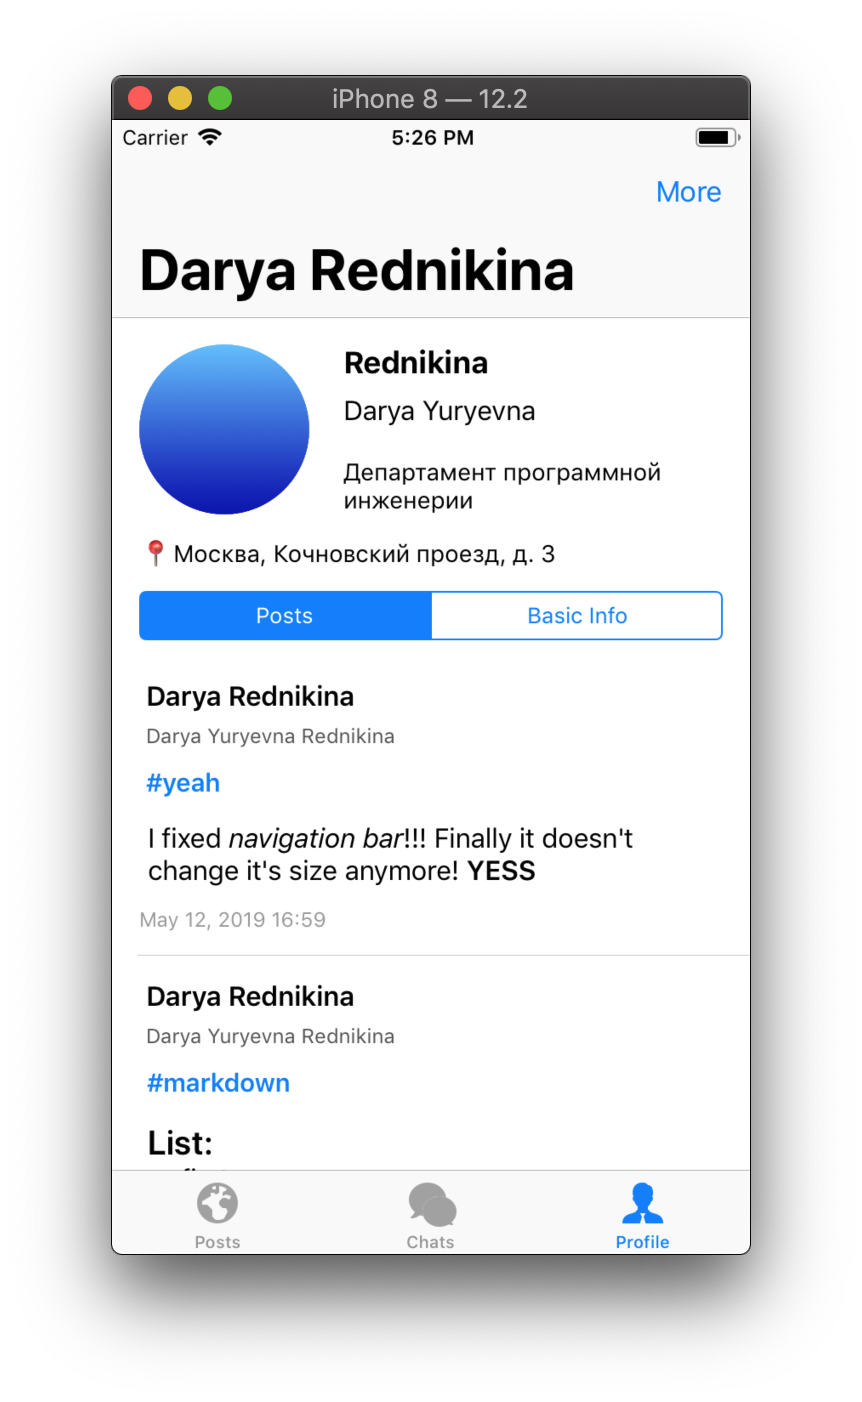
\includegraphics[width=\linewidth]{../includes/pmi/profile.png}
			\caption{\label{pic: mypr} Просмотр профиля}
		\end{subfigure}
		\begin{subfigure}[b]{0.3\linewidth}
			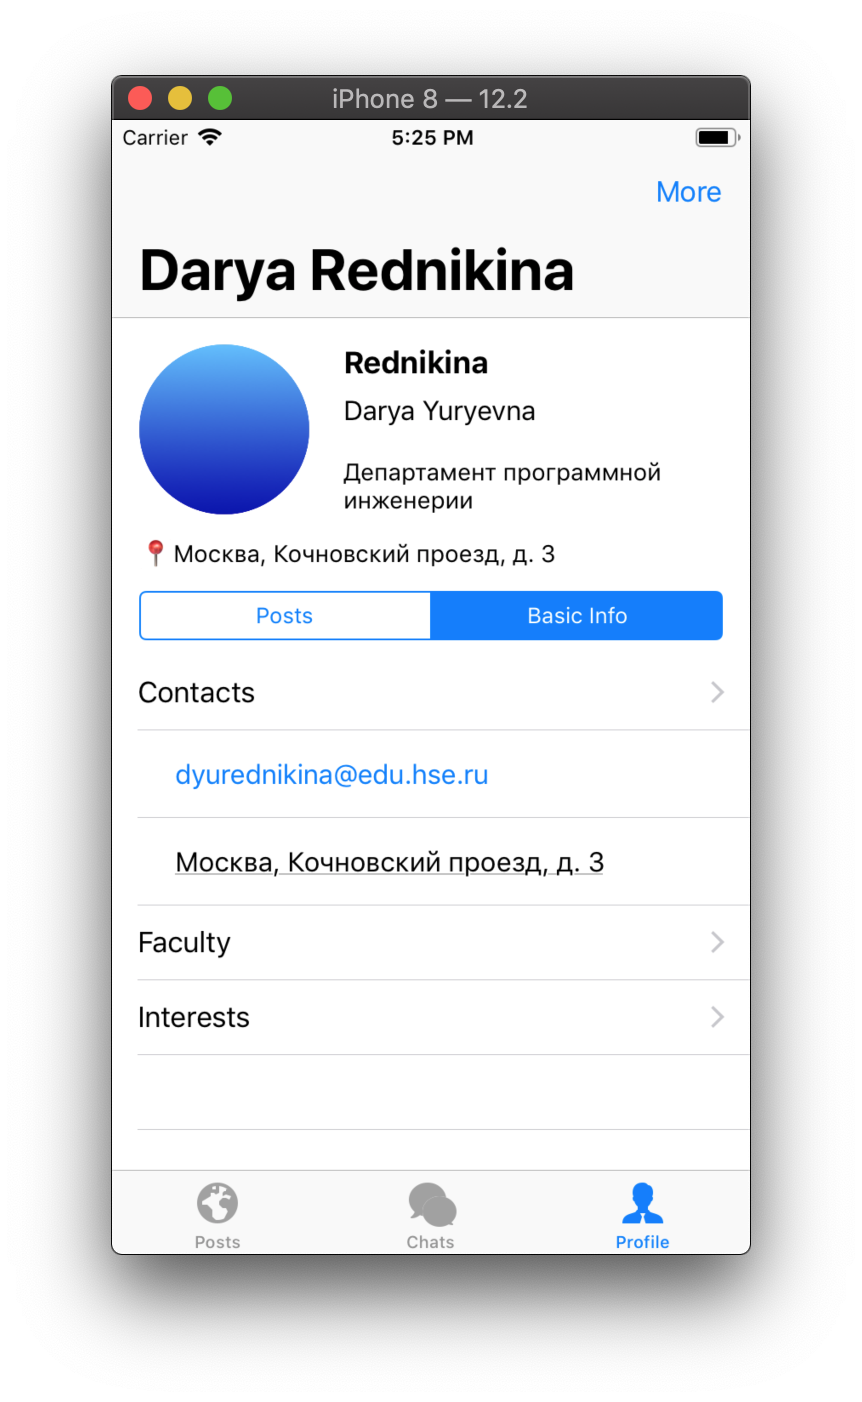
\includegraphics[width=\linewidth]{../includes/pmi/basic_info.png}
			\caption{\label{pic: bi} Базовая информация}
		\end{subfigure}
		\begin{subfigure}[b]{0.3\linewidth}
			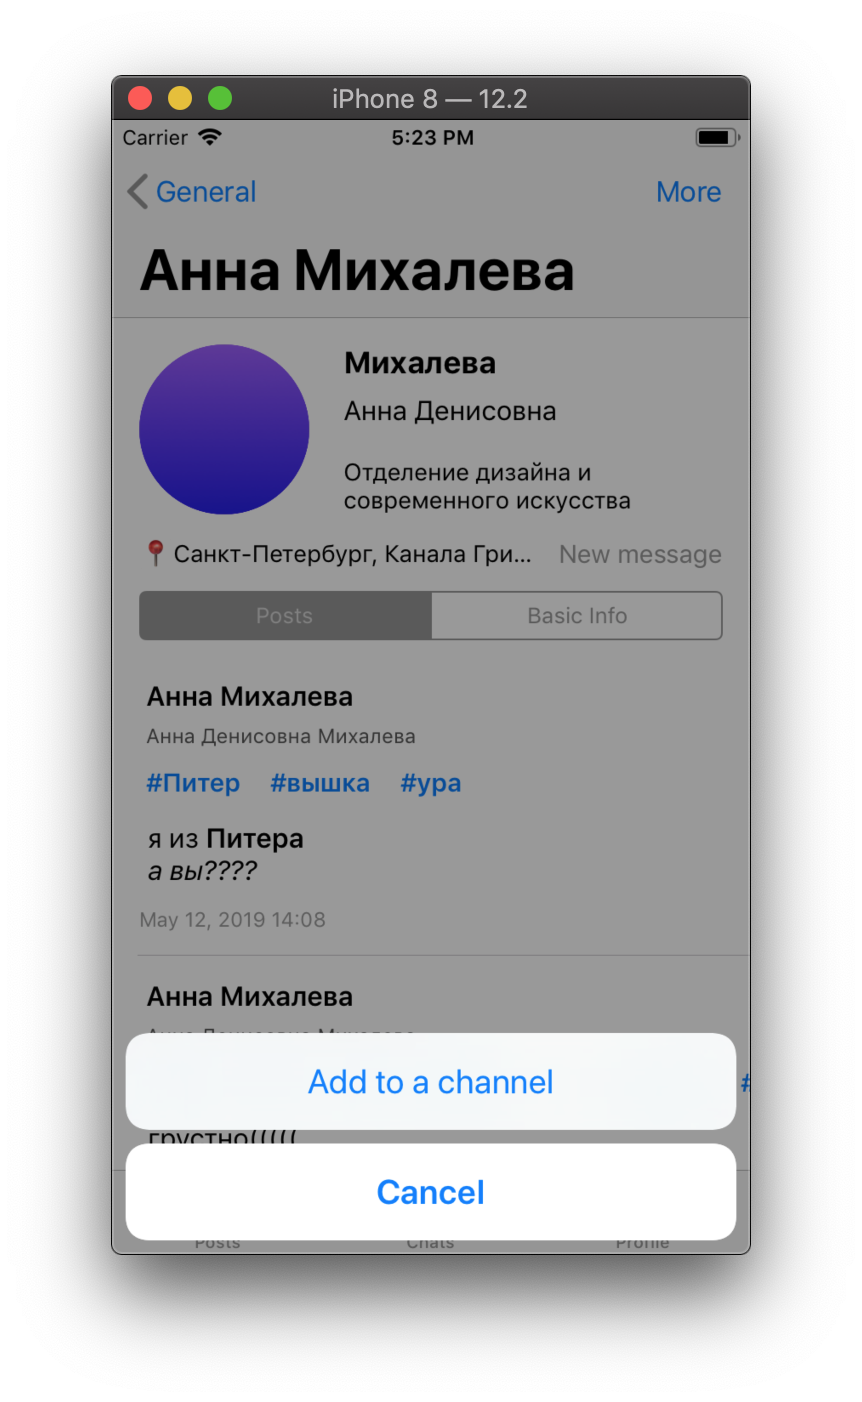
\includegraphics[width=\linewidth]{../includes/pmi/otherprofile_functions.png}
			\caption{\label{pic: otherpr} Опции профиля}
		\end{subfigure}
		
		\caption{\label{pic: myprofile} Просмотр профиля}
	\end{figure}
\clearpage
	\subsubsection{Выход из социальной сети}
	Находясь в секции таббара \textit{Profile}, есть возможность при нажатии справа сверху кнопки \textit{Info} выйти из аккаунта, выбрав <<Log out>> (см. рис \ref{pic: logout}).
	\begin{figure}[h!]
		\centering
		\begin{subfigure}[b]{0.3\linewidth}
			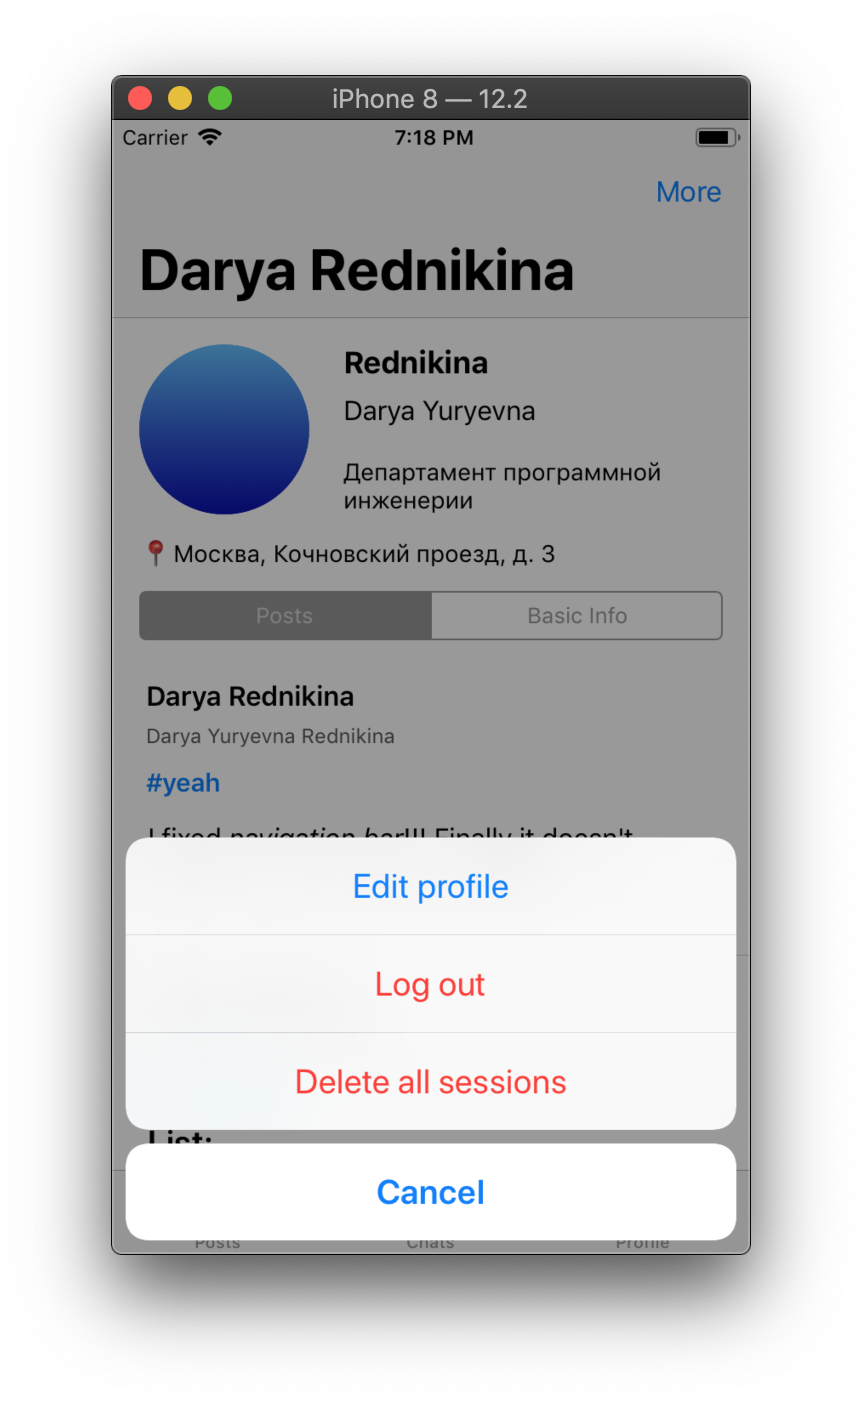
\includegraphics[width=\linewidth]{../includes/pmi/profile_functions.png}
			\caption{\label{pic: logout}Выход из аккаунта}
		\end{subfigure}
	\caption{\label{pic: userOp}Выход}
	\end{figure}
	\newpage
	\section{Сообщения оператору}
	\begin{figure}[h!]
		\centering
		\begin{subfigure}[b]{0.3\linewidth}
			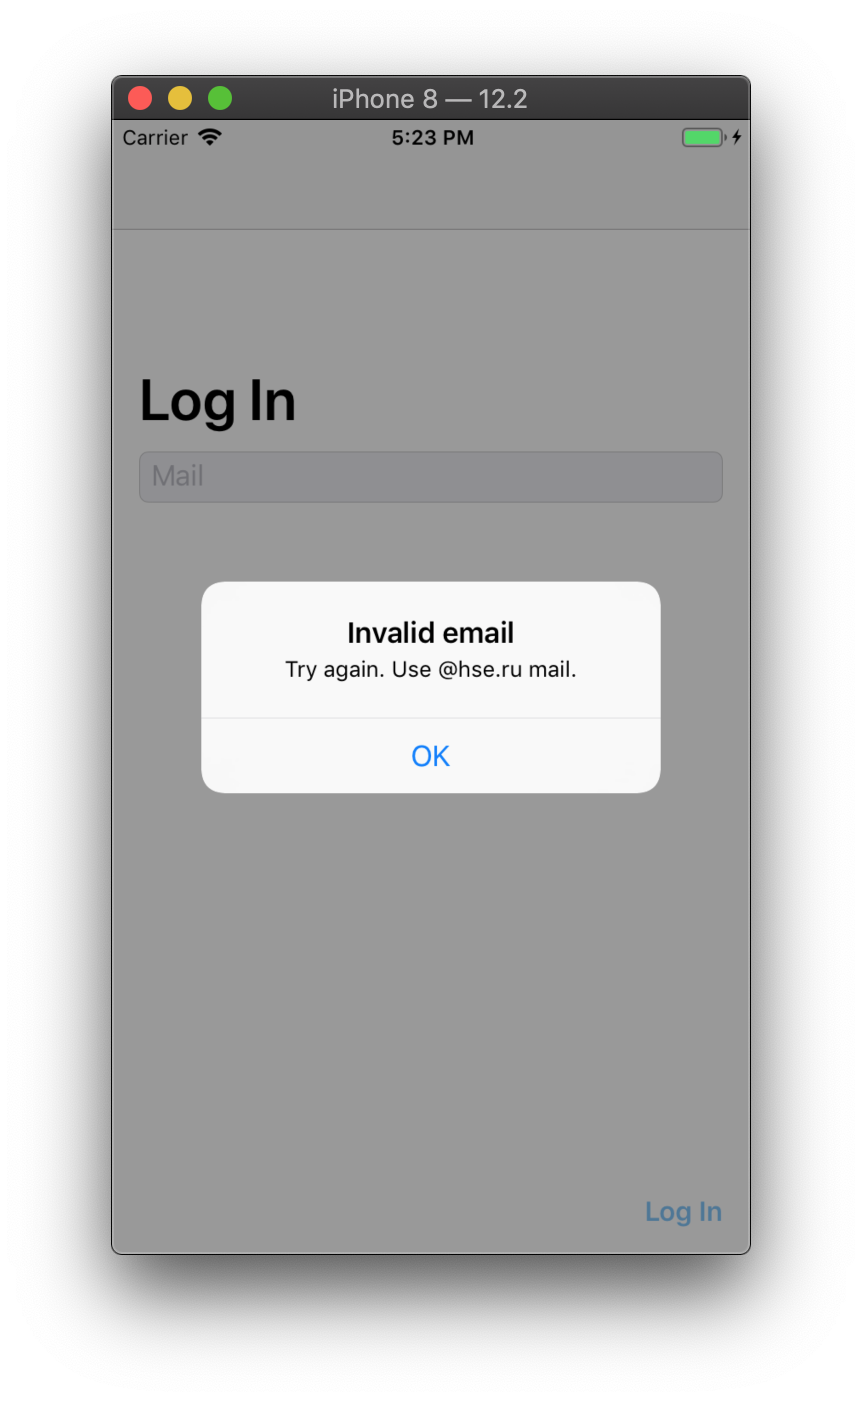
\includegraphics[width=\linewidth]{../includes/ro/invalid.png}
			\caption{\label{pic: invalid} Неверная почта}
		\end{subfigure}
		\begin{subfigure}[b]{0.3\linewidth}
			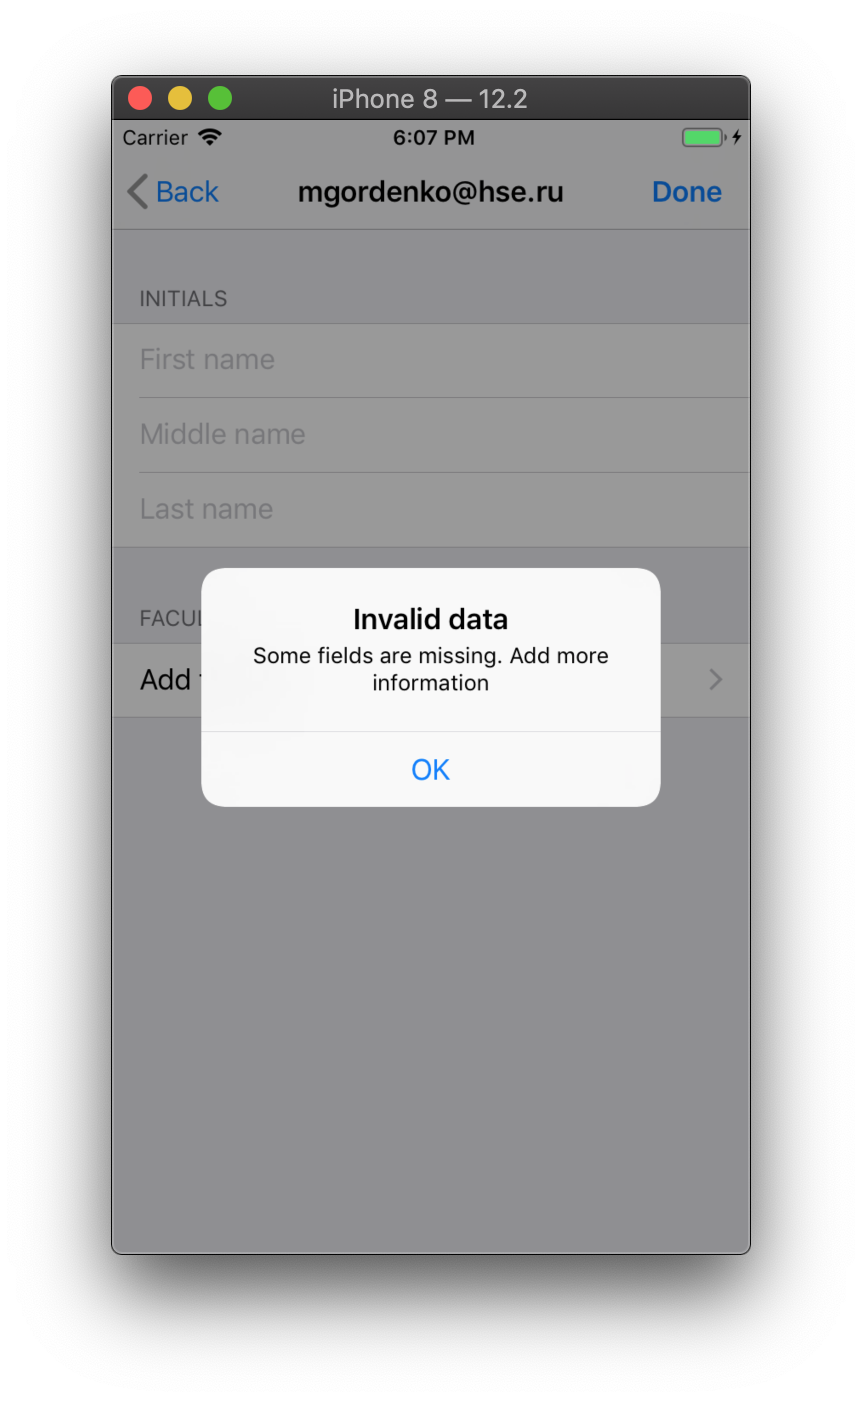
\includegraphics[width=\linewidth]{../includes/ro/invaliddata.png}
			\caption{\label{pic: invaliddata} Неверные данные}
		\end{subfigure}
		\begin{subfigure}[b]{0.3\linewidth}
			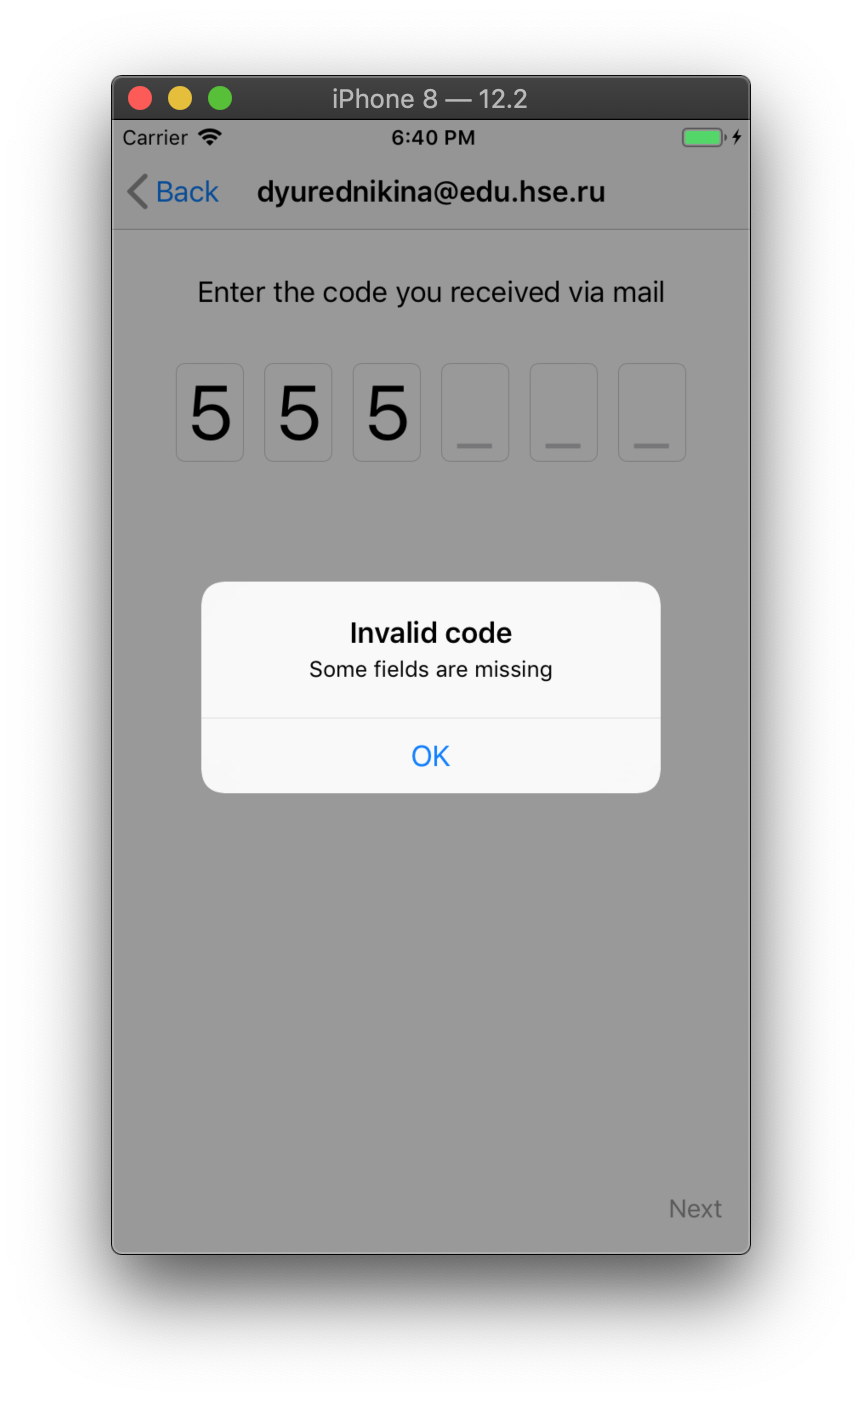
\includegraphics[width=\linewidth]{../includes/ro/wrongcode2.png}
			\caption{\label{pic: wrong_code} Пустые поля}
		\end{subfigure}
		
		\caption{\label{pic: wr} Сообщения оператору}
	\end{figure}
	
	\addition{Используемые понятия и определения}
	\begin{description}
		\item[Социальная сеть] -- это интернет-площадка, сайт, который позволяет зарегистрированным на нем пользователям размещать информацию о себе и коммуницировать между собой, устанавливая социальные связи
		\item[Хэштег] -- ключевое слово или несколько слов сообщения, тег (пометка), используемый в микроблогах и социальных сетях, облегчающий поиск сообщений по теме или содержанию и начинающийся со знака решётки \label{term: hash}
		\item[Пост] -- информационный блок, размещённый пользователем в социальной сети на своей странице и содержащий набор хэштегов, по которым его можно найти \label{term: post}
		\item[Канал] -- сохраненные ранее созданные фильтры новостей (набор хэштегов) по всем публичным постам \label{term: channel}
		\item [Беседа] -- чат для пользователей, в котором одновременно могут присутствовать от 3 до 50 участников \label{term: chat}
		\item [Проект]  -- раздел, в котором сотрудники с любых факультетов по приглашению смогут вместе работать над каким-либо научным исследованием. Проект состоит из timeline (лента с новостями для всех участников проекта) и набором чатов и бесед (с разным количеством участников в каждой) \label{term: project}
		\item [Preview канала]  -- предпросмотр ленты канала с ограничениями на просмотр полной версии поста в ленте, переходом на страницы авторов, нажатия на хэштеги \label{term: preview}
		\item [Preview поста]  -- ограниченный контент (содержание) поста в ленте \label{term: previewPost}
		\item [Model-View-Controller] MVC схема разделения данных приложения, пользовательского интерфейса и управляющей логики на три отдельных компонента: модель, представление и контроллер — таким образом, что модификация каждого компонента может осуществляться независимо
		\item [Xcode] интегрированная среда разработки (IDE) программного обеспечения для платформ macOS, iOS, watchOS и tvOS, разработанная корпорацией Apple
		\item [Dependency manager] программный модуль, который координируют интеграцию внешних библиотек или пакетов в стек приложения
		\item [Constraints] ограничения на размеры и положения объектов на view,  необходимые для правильного определения размеров и позиций контейнеров
		\item [Storyboard] удобный механизм разработки интерфейса программы
	\end{description} %термины и определения
	
	\newpage
	\listRegistration
	%\addcontentsline{toc}{section}{Лист регистрации изменений}
\end{document} % конец документа